

\chapter{Result Analysis}
\label{ch:results}

This chapter outlines what our models produced and what those numbers mean. First
we describe the measures that we used in evaluating performance and the results
of the proposed model, and then decompose the model, layer upon layer, to see
where its performance actually comes from. The remainder of the chapter
turns to the evidence that matters most for this research's central claim: how
the model behaves under a genuine lineage holdout, on a separate collection,
and when the genes it claims to rely on are put to the test.

\section{Performance Evaluation}
\label{sec:perfeval}

The smaller group are the resistant strains, and
even for a single antibiotic only about one in five strains is resistant, so plain
accuracy would not reveal the problem: a model that declared every strain susceptible
would still seem accurate, but would be useless in a clinic. The primary
metric that we are interested in is the area under the precision--recall curve
(PR-AUC), which captures the performance of a model in terms of
precision-recall at all threshold levels and does not encourage a model to
make majority class predictions. It is defined as

\begin{equation}
\text{PR-AUC} = \sum_{n} \left( R_n - R_{n-1} \right) P_n
\end{equation}

where $P_n$ and $R_n$ are the precision and recall at the $n$-th threshold.

We also report a few other measures, since there is no single number which
tells the entire story. Matthews Correlation Coefficient (MCC) employs all
four cells of the confusion matrix simultaneously, and remains truthful in
case of imbalanced classes:

\begin{equation}
\text{MCC} = \frac{TP \times TN - FP \times FN}
{\sqrt{(TP+FP)(TP+FN)(TN+FP)(TN+FN)}}
\end{equation}

MCC can be between $-1$ and $+1$ (where $0$ indicates model guessing), and all
values are calculated per antibiotic using a one-versus-rest approach. F1 is
the harmonic mean of precision and recall; F2 weighted recall four times
higher, since failing to identify a drug-resistant strain is worse than
falsely labelling a susceptible strain resistant (it sends a patient to a drug that will not
work, whereas a false positive just wastes a treatment slot):

\begin{equation}
F_1 = 2 \cdot \frac{P \cdot R}{P + R},
\qquad
F_2 = 5 \cdot \frac{P \cdot R}{4P + R}
\end{equation}

We show accuracy for thoroughness, but we do not use it. Measures of machine
learning are inadequate by themselves to tell a clinician whether a tool is
safe, and so we also report the microbiology vocabulary. A \emph{very major
error} (VME) is a resistant strain called susceptible, which is the
dangerous case; a \emph{major error} (ME) is the reverse, which costs a drug
option but does not put the patient directly at risk; and \emph{categorical
agreement} (CA) is the proportion of strains on which our call matched
the laboratory result. All these evaluations determine three
things: the degree to which the model ranks strains well (PR-AUC), the degree
to which it makes balanced decisions at some threshold (MCC, F1, F2), and
whether its errors would be tolerated in a hospital (VME, ME, CA).

\vspace{1em}

All results in this section use the curated dataset and the random split of
Section~\ref{sec:data}. All measures of all seven antibiotics have been
reported in Table~\ref{tab:main}, and plotted in Figure~\ref{fig:pr_curves} as
a background to the PR-AUC column. That figure also carries the lineage-holdout
curves in red, which belong to Section~\ref{subsec:prevmatch} and should be
ignored for now; they are drawn alongside so that the reader can return to a
single figure once both splits have been introduced. For this section, only the
blue curves are relevant.

\begin{table}[htb]
\centering
\caption{TriLens-MoE-Stack on the random split, per antibiotic.}
\label{tab:main}
\small
\begin{tabular}{|l|r|r|r|r|r|}
\hline
\textbf{Antibiotic} & \textbf{PR-AUC} & \textbf{MCC} & \textbf{F1} & \textbf{F2} & \textbf{Accuracy} \\ \hline
CIP & \textbf{0.9773} & 0.9088 & 0.9282 & 0.9197 & 0.9692 \\ \hline
AMP & 0.9440 & 0.7866 & 0.8932 & 0.8917 & 0.8933 \\ \hline
CTX & 0.9019 & 0.7904 & 0.8173 & 0.8126 & 0.9530 \\ \hline
SXT & 0.8352 & 0.6954 & 0.7875 & 0.7730 & 0.8707 \\ \hline
CAZ & 0.8299 & 0.6928 & 0.7290 & 0.7169 & 0.9356 \\ \hline
AMC & 0.7482 & 0.5237 & 0.6563 & 0.6250 & 0.8035 \\ \hline
GEN & \textbf{0.7037} & 0.6095 & 0.6386 & 0.5915 & 0.9341 \\ \hline
\textbf{Average} & \textbf{0.8486} & \textbf{0.7153} & \textbf{0.7786} & \textbf{0.7615} & \textbf{0.9085} \\ \hline
\end{tabular}
\vspace{0.4em}

\noindent\footnotesize\textit{Note:} Ciprofloxacin has the highest PR-AUC (0.9773) and
gentamicin the lowest (0.7037), the spread the text below discusses; the last row averages
across all seven antibiotics. Bold marks the extreme values of the PR-AUC column, best and
worst alike, and the average row.
\end{table}

\FloatBarrier
\begin{figure}[htb]
\centering
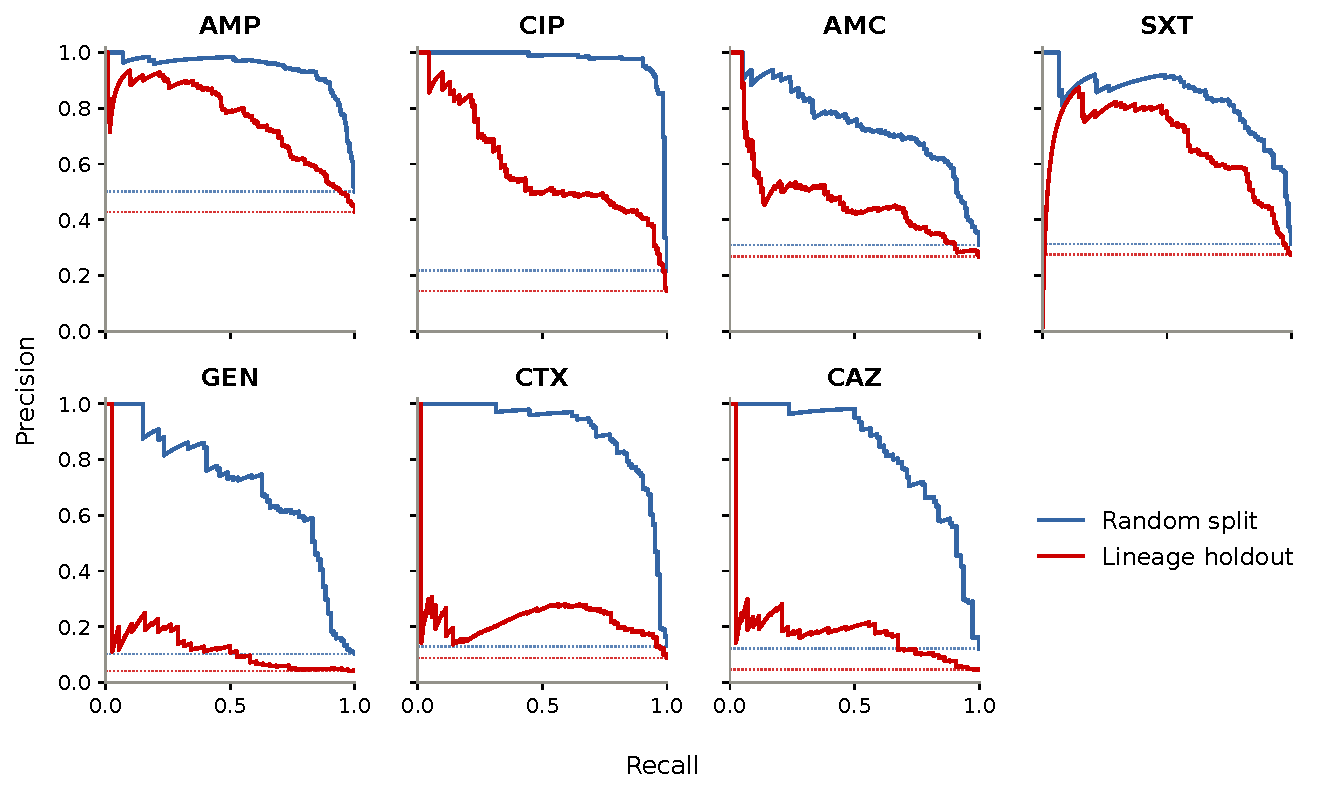
\includegraphics[width=\textwidth]{fig_pr_curves.pdf}
\caption{Precision--recall curves for all seven antibiotics.}
\label{fig:pr_curves}
\fignote{Blue is the random-split test set discussed in this section; red is the
sequence-type lineage holdout, which is not analysed until
Section~\ref{subsec:prevmatch} and is drawn here only so the two can be compared on
one set of axes. The dotted lines are the no-skill baselines, one per split.}
\end{figure}

The average PR-AUC is 0.849, yet the average conceals a broad distribution, and
the interesting part is the spread. The clearest case is ciprofloxacin, at 0.9773 with MCC
0.9088, which is close to a practical ceiling for this kind of data, followed
by ampicillin at 0.9440. On the other hand, gentamicin comes in at 0.7037
and amoxicillin-clavulanate at 0.7482, meaning the spread of best to worst is
nearly 0.27 for models trained on exactly the same genomes with the exact same
architecture.

The accuracy column is different from the others. Gentamicin has the lowest
PR-AUC value, but high accuracy value of 0.9341 as the proportion of strains
resistant to gentamicin is small, so a model can achieve a high accuracy, but
fail to detect many resistant strains. This is the same trap as above, and
the reason accuracy is not our primary measure. As far as a hospital is concerned, it
is the type of error that the model produces, of which the results are
documented in Table~\ref{tab:clinical}.

\FloatBarrier
\begin{table}[htb]
\centering
\caption{Clinical error rates at a threshold of 0.5, ordered by very major error
rate.}
\label{tab:clinical}
\small
\begin{tabular}{|l|r|r|r|l|}
\hline
\textbf{Antibiotic} & \textbf{VME} & \textbf{ME} & \textbf{CA} & \textbf{Meets CLSI limits} \\ \hline
CIP & \textbf{0.086} & 0.015 & 0.969 & No (ME only) \\ \hline
AMP & 0.109 & 0.104 & 0.893 & No \\ \hline
CTX & 0.190 & 0.026 & 0.953 & No (ME only) \\ \hline
SXT & 0.236 & 0.080 & 0.871 & No \\ \hline
CAZ & 0.291 & 0.033 & 0.936 & No \\ \hline
AMC & 0.394 & 0.108 & 0.804 & No \\ \hline
GEN & \textbf{0.436} & 0.023 & 0.934 & No (ME only) \\ \hline
\end{tabular}
\vspace{0.4em}

\noindent\footnotesize\textit{Note:} Ciprofloxacin has the lowest very major error (VME) rate at
0.086 and gentamicin the highest at 0.436. No antibiotic meets both CLSI limits at once;
``No (ME only)'' means only the major-error limit is met.
\end{table}

Ciprofloxacin reappears as the strongest, having a VME of 0.086, and a
categorical agreement of 0.969. Gentamicin is weakest with 0.436 (almost half
of all resistant strains would be reported sensitive) and
amoxicillin-clavulanate is almost as poor (0.394). The ordering is important,
as an almost identical ordering is rediscovered under the lineage holdout in
Section~\ref{subsec:prevmatch} in an entirely different way.

\vspace{1em}

The categorical agreement column is the same as the accuracy column of
Table~\ref{tab:main}, and this is not by chance. During data preparation
the intermediate results were grouped with the resistant results, so the
intermediate category no longer exists in this dataset. Categorical
agreement therefore reduces to binary accuracy here.
Gentamicin illustrates this point clearly, with a categorical agreement of 0.934 versus
a VME of 0.436. On the same strains, the same model is seen to be strong by
one measure and unusable by the other.

\vspace{1em}

The CLSI limits require both the VME and ME rates to stay under three
percent. Three antibiotics satisfy the major error limit, which are
ciprofloxacin at 0.015, gentamicin at 0.023 and cefotaxime at 0.026 but none
satisfy the very major error limit, therefore, the model is not yet prepared
to be used as a diagnostic test.

\vspace{1em}

The obvious response is that the fixed 0.5 threshold was never tuned to
clinical cost, and that the numbers above could be an artefact of positioning
the cut. To do this, we trained a threshold for each antibiotic on the
validation set, constraining the $F_2$ objective of Equation~\eqref{eq:fbeta}
and capping the major error rate, and assessed each on the test set. While the
tuning for $F_2$ moves the mean very major error rate only from 0.249 to
0.210, still far above the limit of 0.03, and forcing the major error rate to
remain inside the limit pushes the mean very major error rate to 0.437,
neither rescues the model. In fact, none of the antibiotics was able to achieve both
thresholds at any threshold value that we tested, because shifting the cut
trades one kind of error against the other instead of
cutting down on both. It is not the position of the cut that drives the clinical
shortfall, however, but the model's ability to separate the two classes, a point
the heritability comparison in Section~\ref{subsec:published} also supports. As
such, future work should not focus on calibration, but on the feature
representation.

\FloatBarrier
\section{Analysis of Design Solutions}
\label{subsec:layerabl}

Each neural lens reads a different part of the genome and a gate determines
the trustworthiness of each lens, with five classical learners combined by a
stacking layer. To determine whether each part is warranted, we removed each
component in turn and measured the impact on performance. We trained three variants using the same data,
seed and test set.

\begin{itemize}
  \item \textbf{Stage 1.} The three lenses only. They average their outputs
  with equal weighting. No gate is used.
  \item \textbf{Stage 2.} The three lenses and the mixture-of-experts gate,
  such that the model learns the extent to which to rely on individual lenses
  on individual samples and antibiotics. This is the neural part of the model
  on its own.
  \item \textbf{Stage 3.} The complete model in which the neural output is
  appended with the five classical base learners via the meta-learner.
\end{itemize}

Table~\ref{tab:ablation} sets the three variants side by side, per antibiotic, with the gain
each stage adds over the one before it. Reading down a column shows how much of a drug's final
score was already in place before the classical learners were attached to it.

\begin{table}[htb]
\centering
\caption{Component ablation on the random split, with the PR-AUC gain each added
part contributes over the stage before it.}
\label{tab:ablation}
\small
\setlength{\tabcolsep}{3pt}
\resizebox{\textwidth}{!}{%
\begin{tabular}{|l|r|r|r|r|r|r|r|r|r|}
\hline
\textbf{Stage} & \textbf{AMP} & \textbf{CIP} & \textbf{AMC} & \textbf{SXT} & \textbf{GEN} & \textbf{CTX} & \textbf{CAZ} & \textbf{Avg} & \textbf{Gain} \\ \hline
Stage 1: lenses only    & 0.8920 & 0.9248 & 0.6249 & 0.7217 & 0.5168 & 0.8103 & 0.7267 & 0.7453 & N/A \\ \hline
Stage 2: + MoE gate     & 0.8970 & 0.9489 & 0.6347 & 0.7453 & 0.5835 & 0.8659 & 0.7893 & 0.7807 & +0.0353 \\ \hline
Stage 3: + stacking     & 0.9440 & 0.9773 & 0.7482 & 0.8352 & 0.7037 & 0.9019 & 0.8299 & \textbf{0.8486} & \textbf{+0.0679} \\ \hline
\end{tabular}
}
\vspace{0.4em}

\noindent\footnotesize\textit{Note:} The full model reaches an average PR-AUC of 0.8486;
classical stacking adds +0.0679 over stage 2, about twice the gate's own +0.0353 contribution.
\end{table}
\FloatBarrier

There are two points that are established. First, there is no dead weight: for
each and every antibiotic, the performance improves when it goes from Stage 1
to Stage 2 and then to Stage 3. Second, the parts do not aid equally.
Combining neural predictions with classical learners achieves on average
about 0.0679 more than the neural design alone, while the gate achieves only
0.0353. The neural lenses are useful, but not sufficient by themselves, and
thus the final model is best referred to as a hybrid rather than as a neural
model. Figure~\ref{fig:layer_ablation} breaks the same three stages down antibiotic by
antibiotic.

\begin{figure}[htb]
\centering
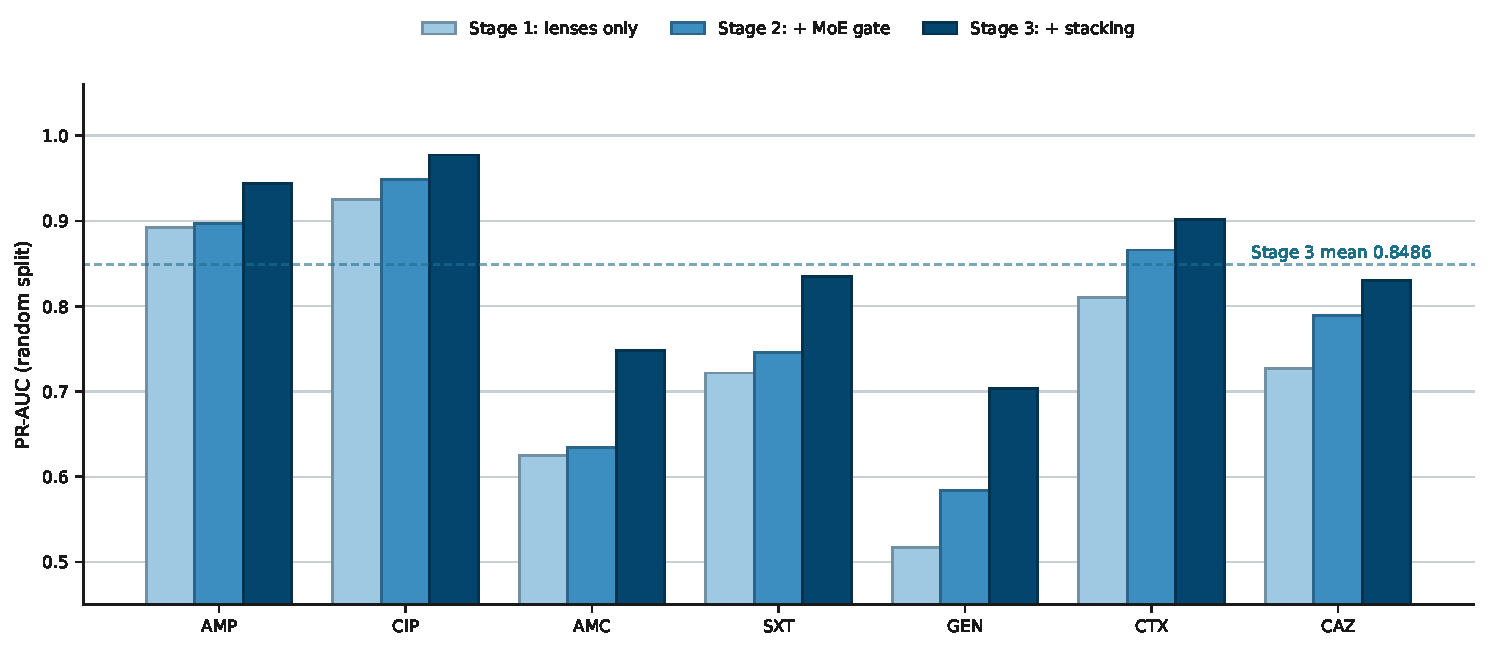
\includegraphics[width=\textwidth]{fig_layer_ablation.pdf}
\caption{The component ablation of Table~\ref{tab:ablation}, per antibiotic.}
\label{fig:layer_ablation}
\fignote{Every antibiotic improves from Stage 1 to Stage 2 and again from Stage 2 to
Stage 3, but the size of each step varies widely; gentamicin gains most from the
classical stacking layer.}
\end{figure}

The average weight assigned to each lens by the gate is shown in
Table~\ref{tab:gate}, and the weights by antibiotic in
Figure~\ref{fig:gate_routing}.

\begin{table}[htb]
\centering
\caption{Average gate weights on the test set. Each row sums to one.}
\label{tab:gate}
\small
\resizebox{\textwidth}{!}{%
\begin{tabular}{|l|r|r|r|}
\hline
\textbf{Antibiotic} & \textbf{Lens A (motif CNN)} & \textbf{Lens B (presence/absence)} & \textbf{Lens C (cross-antibiotic)} \\ \hline
AMP & 0.070 & 0.852 & 0.078 \\ \hline
CIP & \textbf{0.035} & 0.590 & 0.374 \\ \hline
AMC & 0.095 & 0.742 & 0.163 \\ \hline
SXT & 0.052 & \textbf{0.900} & 0.047 \\ \hline
GEN & 0.098 & 0.731 & 0.171 \\ \hline
CTX & 0.064 & 0.815 & 0.121 \\ \hline
CAZ & 0.044 & 0.835 & 0.122 \\ \hline
\end{tabular}
}
\vspace{0.4em}

\noindent\footnotesize\textit{Note:} Ciprofloxacin's Lens A weight of 0.035 is the lowest in the
table despite being the drug that lens was built for, and trimethoprim-sulfamethoxazole's Lens B
weight of 0.900 is the highest, closest to gate collapse; both are discussed below.
\end{table}

The trend is the same. Most of the weight of each antibiotic, 0.590 to 0.900,
is in Lens B, which reads which genes are present or absent, whereas Lens A,
the convolutional lens reading mutation patterns within genes, never goes
above 0.098. At least this is consistent with the biology as a large part of
the resistance in \textit{E. coli} is conferred by acquired genes.

\begin{figure}[htb]
\centering
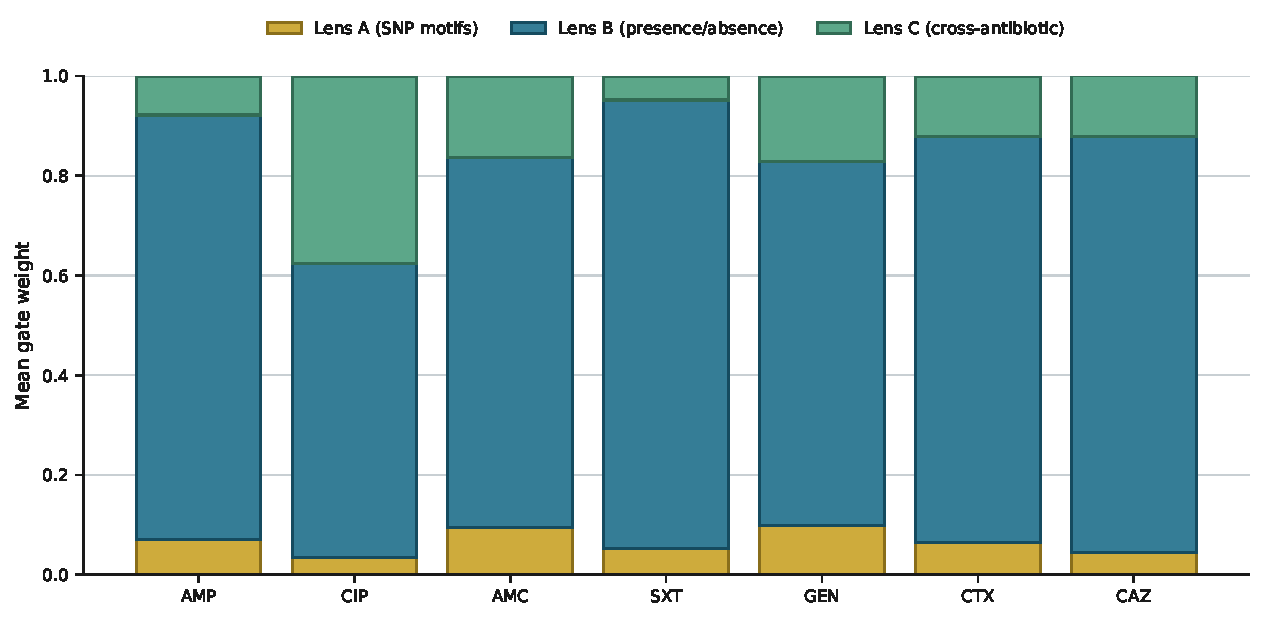
\includegraphics[width=\textwidth]{fig_gate_weights.pdf}
\caption{Mean gate weight assigned to each lens, by antibiotic, on the test set.}
\label{fig:gate_routing}
\fignote{The three weights sum to one for each antibiotic; these are the values of
Table~\ref{tab:gate} drawn as stacked bars.}
\end{figure}

\vspace{1em}

Ciprofloxacin is where the table stops agreeing with the design. The rationale
for the gate in Section~\ref{subsec:moegate} is a prediction: a drug whose
resistance is based on an acquired gene should route to Lens B, whereas a drug
whose resistance is based on a point mutation in a target enzyme should route
to Lens A. Ciprofloxacin is the most obvious point-mutation drug that we have
in our panel, and the one that our SHAP analysis suggests is related to
\textit{gyrA} and \textit{parC}; yet Lens A receives 0.035 for this drug, the
lowest value in the table. The prediction fails on the one antibiotic where it
was most testable. This is the highest value for Lens C, but it is difficult
to read from either direction. The lens shares drug-class head evidence, but
ciprofloxacin is the only fluoroquinolone in the panel and has no same-class
partner, and although its co-resistance refinement step may still link
ciprofloxacin to ceftazidime, which shares $\phi = 0.52$ in this collection
(Figure~\ref{fig:coresistance}), that is co-occurrence rather than
mechanism. On neither reading can 0.374 be taken as the gate finding the
mechanism.

\vspace{1em}

The gate hence informs us of the lens the model inclines on, which is
interesting to know, but its routing is not in the direction which the design
supposed. The same conclusion is drawn in the attention audit in
Section~\ref{subsec:attnfix}. A second reading of the table points the same
way. In the fold reported in Section~\ref{subsec:devadjust}, Lens B takes a
weight of 0.895. The other two lenses are pushed to virtually zero. This is
exactly the pattern the entropy penalty is meant to prevent. In the final
weights, trimethoprim-sulfamethoxazole reaches 0.900, even higher than that
fold. Three more drugs sit above 0.81: ampicillin at 0.852, ceftazidime at
0.835, and cefotaxime at 0.815. It seems
that the penalty would have slowed, but not stopped, collapse, and therefore,
these weights are possibly associated with optimisation-like dynamics as well
as with biology.

\FloatBarrier
\section{Final Design Adjustments}
\label{sec:designadj}

\FloatBarrier
\subsection{The Change of Dataset}
\label{subsec:ownprep}

An earlier phase of the project created its own set of features out of the
raw variant files. Filtering of variants was done by missingness and
frequency, followed by coding into binary columns and merging with the
phenotype table. This resulted in a 6{,}962 by 80{,}984 strain-by-feature
matrix. The screening of
various model families on it revealed two issues that were not related to the
models themselves: namely, our filtering criteria discarded variants based on
simple thresholds and no gene-level structure was present, which is precisely
what the proposed model reads. We thus relocated to the curated version
releases of Arcadia Science that had been previously quality checked and
mapped to genes, and all the experiments described in this research have used
that dataset.

The weakest of the families we tried was a one dimensional convolutional
network, and not merely because it needed tuning, but because a convolution
expects neighbouring columns to be related: those columns should have held
variants from nearby positions, whereas in the file the adjacent columns of
the matrix held variants from unrelated positions in the genome. The latter, one of our clearer
findings, is directly tested in Section~\ref{subsec:cnnfail} when we apply
that explanation to the curated data.

\FloatBarrier
\subsection{Adjustments Made During Development}
\label{subsec:devadjust}

Four further pieces of the final design came from problems encountered during
development rather than in planning. We had intended to have an entirely neural model. The ablation in
Section~\ref{subsec:layerabl} altered that: the neural lenses alone attained
0.7807 and including the classical learners boosted the model up to 0.8486,
thus, dropping them would have cost 0.068 to maintain the cleanliness of the
design. Second, the gate occasionally shifted to assigning a single lens
nearly the entire weight, such as 0.895 on Lens B in one of the
cross-validation folds and the other two almost on the lower end, when the
model is no longer a mixture of experts. To avoid this, we added a penalty term to the training loss based on the
entropy of the gate weights: it rises automatically as the weights become too
concentrated on a single lens, discouraging such a collapse. After this
penalty was applied, the weights recovered within two or three epochs.

\vspace{1em}

Third, Lens B computes attention over more than 32{,}000 genes with the absent
genes masked out, and in half precision this becomes invalid, because the
softmax breaks down over that many masked entries. Calculating just one softmax with single precision, with
the rest of the model in mixed precision, eliminated the problem with
virtually no performance penalty. Fourth, our first baseline reduced the SNP
matrix to 1024 principal components which was quick but lost the connection
between the SNP and the gene and we had a score of 0.803; all later models
were based on the gene-level view, which got us to 0.830.

\FloatBarrier
\section{Statistical Analysis}
\label{sec:statanalysis}

In our test set there are 1{,}045 strains and in some antibiotics there are
only a few hundred of known label, so one or two points difference can be
simply accidental. We resampled the test set (1{,}000 bootstrap resamples with
replacement) to recalculate PR-AUC, and used the 2.5th and 97.5th percentiles
as a 95\% confidence interval. The result is shown in Table~\ref{tab:ci} and
plotted in Figure~\ref{fig:ci_forest} as the intervals against the no-skill
baseline of the individual drugs, i.e., the range within which the raw scores
are most misleading: a PR-AUC has to be read against the prevalence of the
drug it represents, not against the other drugs in the column. The PR-AUC of
ampicillin, 0.944, sits above a no-skill baseline of roughly one resistant
strain in two. The score of gentamicin, 0.7037, appears smaller in absolute
terms, but its no-skill baseline is only about one resistant strain in ten.
Gentamicin's raw score is lower, yet it is the greater gain over chance.

\begin{table}[htb]
\centering
\caption{Bootstrap confidence intervals for the proposed model on the random-split
test set, from 1{,}000 resamples.}
\label{tab:ci}
\small
\begin{tabular}{|l|r|l|}
\hline
\textbf{Antibiotic} & \textbf{PR-AUC} & \textbf{95\% confidence interval} \\ \hline
AMP & 0.9440 & [0.919, 0.965] \\ \hline
CIP & 0.9773 & \textbf{[0.961, 0.990]} \\ \hline
AMC & 0.7482 & [0.680, 0.809] \\ \hline
SXT & 0.8352 & [0.773, 0.891] \\ \hline
GEN & 0.7037 & \textbf{[0.612, 0.786]} \\ \hline
CTX & 0.9019 & [0.851, 0.943] \\ \hline
CAZ & 0.8299 & [0.762, 0.882] \\ \hline
\textbf{Average} & \textbf{0.8486} & \\ \hline
\end{tabular}
\vspace{0.4em}

\noindent\footnotesize\textit{Note:} Ciprofloxacin's interval, [0.961, 0.990], is the tightest in
the table, backed by the most labelled data; gentamicin's, [0.612, 0.786], is the widest,
backed by the least. Bold marks the extreme values in a column, best and worst alike.
\end{table}

Gentamicin ranges 0.612 to 0.786, a range of nearly
0.18, and this is simply the result of few resistant strains, but
ciprofloxacin, which has more labelled strains and a stronger signal, has a
much smaller range. Any difference between two models on this test set must
therefore exceed this interval width before it can be termed significant.
None of the differences reported in this chapter between closely related
methods clears that bar. Figure~\ref{fig:ci_forest} plots the same intervals against
each antibiotic's no-skill baseline.

\begin{figure}[htb]
\centering
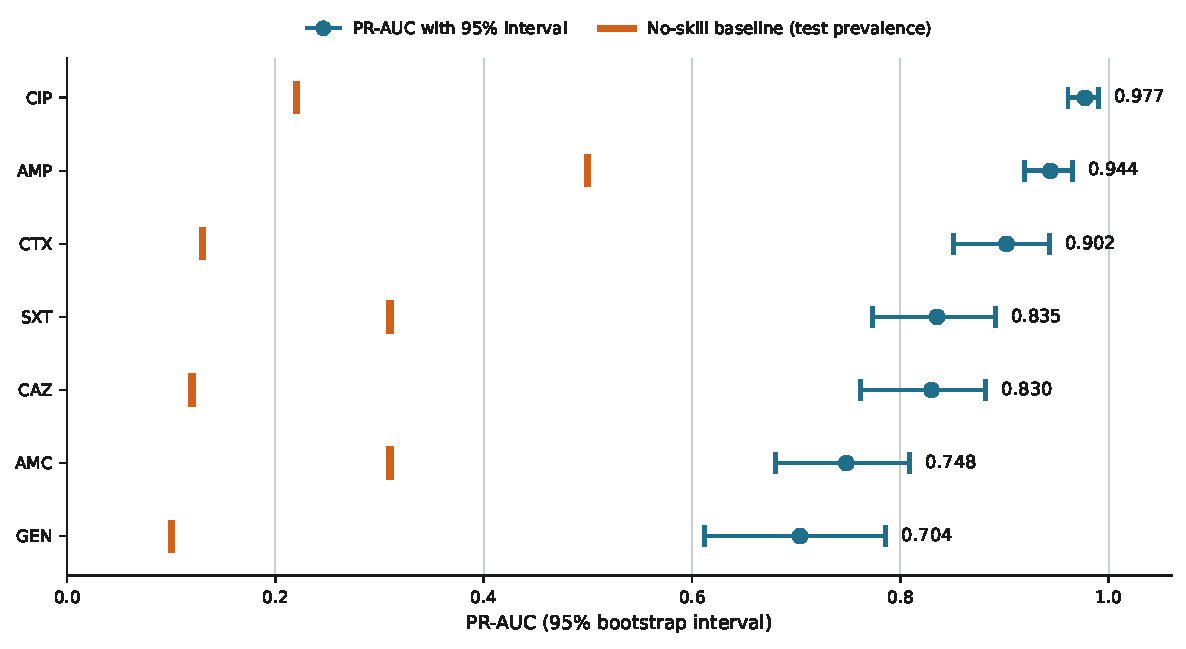
\includegraphics[width=\textwidth]{fig_ci_forest.pdf}
\caption{PR-AUC with 95\% bootstrap intervals, against each antibiotic's no-skill
baseline.}
\label{fig:ci_forest}
\fignote{The no-skill baseline is the test-set prevalence for that antibiotic.}
\end{figure}

\vspace{1em}

Table~\ref{tab:baselines} distinguishes between two similar but different
questions. The first is the comparison of the proposed model with external
models. There are three external baselines: a null model using only the
phylogroup label, TabNet and the gradient-boosting model using PCA components
that this project began with. The second question is what each component of the
proposed system contributes to the overall result. With this in mind, the five
base learners are tested individually as well. But these are not external
baselines. The proposed system consists of multiple learners, each feeding the
meta-learner. Thus, comparing these learners with the full system is not an
external comparison, but rather an ablation. All models were evaluated with the
same data splits and the same five-fold protocol. The values reported are the
mean PR-AUC scores of the seven antibiotics, and Figure~\ref{fig:baseline_ladder}
draws every row of the table on both splits at once.

\begin{table}[htb]
\centering
\caption{Comparisons of the proposed model with external baselines and results of
the component models. The phylogroup-only and PCA baselines were not evaluated
with the lineage holdout.}
\label{tab:baselines}
\small
\resizebox{\textwidth}{!}{%
\begin{tabular}{|l|r|r|}
\hline
\textbf{Model} & \textbf{PR-AUC, random split} & \textbf{PR-AUC, lineage holdout} \\ \hline
\multicolumn{3}{|l|}{\textit{External baselines}} \\ \hline
Phylogroup label only (null baseline) & 0.2914 & not run \\ \hline
TabNet, tabular deep learning baseline & 0.6951 & 0.3255 \\ \hline
XGBoost on 1{,}024 PCA components & 0.8033 & not run \\ \hline
\multicolumn{3}{|l|}{\textit{Components of the proposed system, each on its own}} \\ \hline
Random Forest, gene features & 0.7809 & 0.4931 \\ \hline
Logistic Regression, gene features & 0.7923 & 0.4408 \\ \hline
LightGBM, gene features & 0.8338 & 0.5516 \\ \hline
XGBoost, gene features & 0.8375 & 0.5507 \\ \hline
XGBoost, chi-squared filtered SNPs & 0.8400 & 0.6299 \\ \hline
\multicolumn{3}{|l|}{\textit{Proposed}} \\ \hline
\textbf{TriLens-MoE-Stack} & \textbf{0.8486} & \textbf{0.6337} \\ \hline
\end{tabular}
}
\vspace{0.4em}

\noindent\footnotesize\textit{Note:} The last row is the proposed model, the one every other row
in the table is being measured against.
\end{table}

\begin{figure}[htb]
\centering
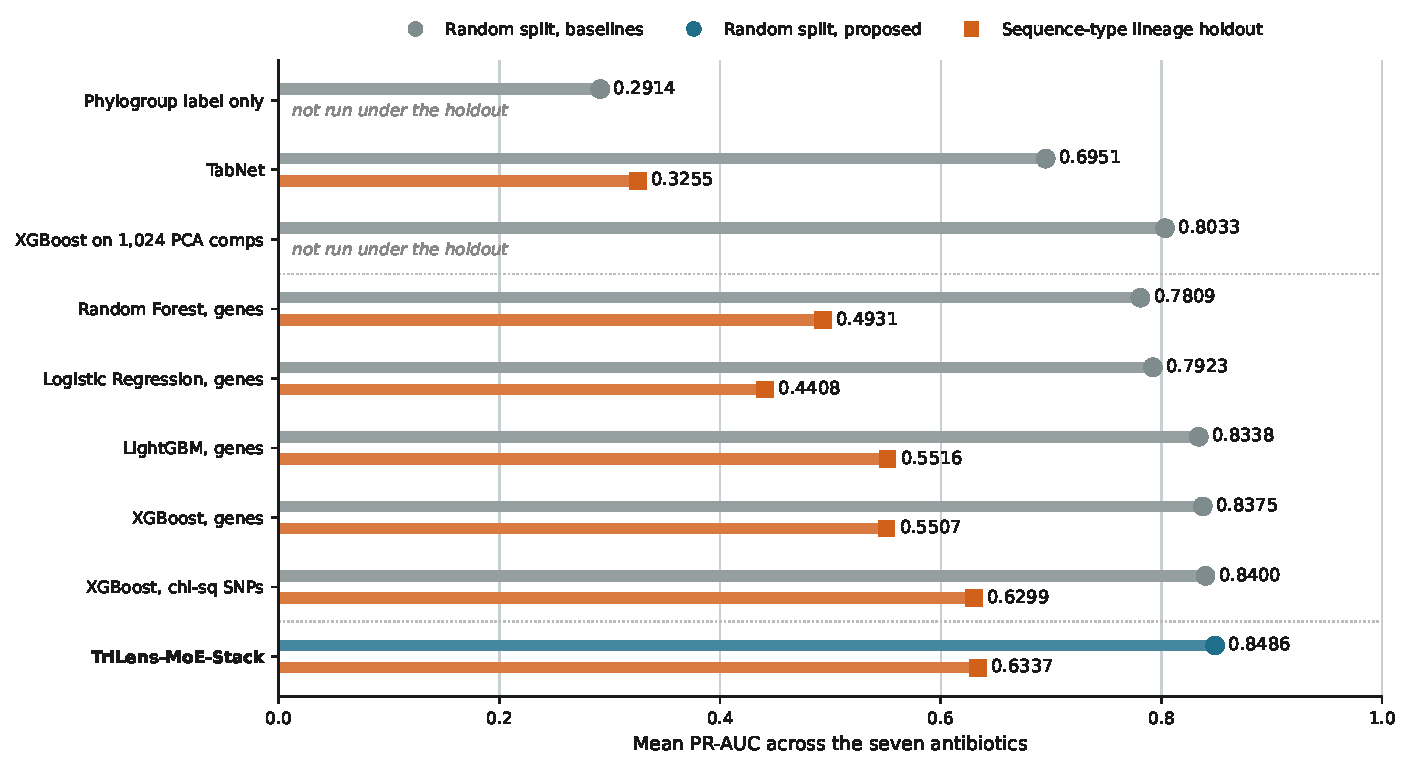
\includegraphics[width=\textwidth]{fig_baseline_ladder.pdf}
\caption{Every model of Table~\ref{tab:baselines} on both splits.}
\label{fig:baseline_ladder}
\fignote{The proposed model leads on the random split, but under the lineage holdout
the whole field compresses into a narrow band and the separation between methods
largely disappears.}
\end{figure}

On the random split the model produces the highest score of all entries in
the table. If only the eight-way phylogroup label is used as a baseline, the
PR-AUC reaches just 0.2914, almost equal to the average frequency of
resistance across the drugs, which is effectively the floor for this task.
The specialized tabular deep-learning baseline, TabNet, achieves only 0.6951,
behind every single classical learner, and falls to 0.3255 under the lineage
holdout, where even the weakest classical learner still reaches 0.4408: added
depth does not help on this problem under either test. The five classical
learners themselves range from PR-AUC 0.7809 to 0.8400, with the three
gradient-boosting models on the higher end of that span. The highest entry in the table, at 0.8486,
is TriLens-MoE-Stack, which leads every external baseline on the average and is ahead of
its own strongest component on five of the seven antibiotics. The
baselines are reported on PR-AUC as a single variable since this is what the
stacking pipeline reported about each learner when in isolation.

\vspace{1em}

It is not just the direction of the result that matters, but also the size of the
improvement. The proposed model outperforms the PCA baseline by 0.0453, TabNet by
0.1535 and the null model by 0.5572. The PCA comparison is the most telling as it
demonstrates what this project contributed, since this project began with the PCA
model. For individual antibiotics, the proposed model has scores above the upper
limit of the baseline interval for ampicillin, ciprofloxacin and
trimethoprim-sulfamethoxazole. Its score is within the interval for the other four
antibiotics. The greatest increase is for trimethoprim-sulfamethoxazole, which
goes from 0.7100 to 0.8352. But there is no benefit for amoxicillin-clavulanate.
This confirms the previous discovery that this is the antibiotic the model knows
the least about.

\vspace{1em}

The five base learners measure different things. The strongest learner gets 0.8400
by itself and the full system gets 0.8486. The difference is minimal at 0.009,
within the bootstrap intervals in Table~\ref{tab:ci}. This means that, as an
ablation result, the stacking layer provides a small improvement on top of the
best component. But this outcome does not mean that the system outperforms an
external method. A comparison of the full system with this component for each
antibiotic on each data split is provided in Table~\ref{tab:vsraw}.

\begin{table}[htb]
\centering
\caption{Comparison of the proposed model with its best single component, the
chi-squared filtered XGBoost, for each antibiotic. The antibiotics are sorted by
the gain on the random split.}
\label{tab:vsraw}
\small
\resizebox{\textwidth}{!}{%
\begin{tabular}{|l|r|r|r|r|r|r|}
\hline
& \multicolumn{3}{c|}{\textbf{Random split}} & \multicolumn{3}{c|}{\textbf{Lineage holdout}} \\ \hline
\textbf{Drug} & \textbf{XGB, $\chi^2$} & \textbf{Proposed} & \textbf{Gain} & \textbf{XGB, $\chi^2$} & \textbf{Proposed} & \textbf{Gain} \\ \hline
CAZ & 0.7951 & 0.8299 & $+0.035$ & 0.5180 & 0.4930 & $\mathbf{-0.025}$ \\ \hline
CTX & 0.8846 & 0.9019 & $+0.017$ & 0.6569 & 0.6073 & $\mathbf{-0.050}$ \\ \hline
SXT & 0.8183 & 0.8352 & $+0.017$ & 0.7609 & 0.7872 & $+0.026$ \\ \hline
AMP & 0.9432 & 0.9440 & $+0.001$ & 0.8910 & 0.9043 & $+0.013$ \\ \hline
CIP & 0.9770 & 0.9773 & $+0.000$ & 0.9348 & 0.9118 & $\mathbf{-0.023}$ \\ \hline
AMC & 0.7490 & 0.7482 & $\mathbf{-0.001}$ & 0.4704 & 0.4865 & $+0.016$ \\ \hline
GEN & 0.7128 & 0.7037 & $\mathbf{-0.009}$ & 0.1777 & 0.2457 & $+0.068$ \\ \hline
\textbf{Average} & \textbf{0.8400} & \textbf{0.8486} & $\mathbf{+0.009}$ & \textbf{0.6299} & \textbf{0.6337} & $\mathbf{+0.004}$ \\ \hline
\end{tabular}
}
\vspace{0.4em}

\noindent\footnotesize\textit{Note:} Bold marks the negative gains, where the full system loses
to its own best component: two drugs on the random split and three under the lineage holdout.
Every one of these differences is smaller than the bootstrap interval, so they indicate a
direction rather than a stable ranking.
\end{table}

The full system is more effective on five out of seven antibiotics on the random
split. The gain is more than 0.01 for three antibiotics: 0.035 for ceftazidime,
0.017 for cefotaxime, and 0.017 for trimethoprim-sulfamethoxazole. The difference
for ampicillin and ciprofloxacin is less than 0.001, meaning that they are
virtually the same. These antibiotics already have a score of 0.94 and 0.98 for
the single component, so there is not much room to improve. With the lineage
holdout the pattern changes. In this instance the entire system is more effective
against four antibiotics. Gentamicin has a gain of 0.068, the highest gain of any
individual antibiotic in this research. It is also the antibiotic on which the
single component has the lowest performance with a score of 0.1777. Ceftazidime
has the reverse trend. It gains most on the random split but it loses 0.025 under
the lineage holdout. All these individual differences are smaller than the
bootstrap interval. So they indicate the direction of the results, but do not
suggest a definite and stable ranking.

\vspace{1em}

The holdout column is a little less encouraging. The strongest single
classical learner reaches 0.6299 compared to 0.6337 for the full model, only a
gap of 0.004, but far less than the bootstrap uncertainty interval around
either value. This is the most unambiguous one-line answer to what this
research has discovered: none of the methods here stand out clearly from others
when lineage relatedness is not taken into account. Neither the ensemble nor
the hybrid design buys anything on unfamiliar strains, and all other analyses in
this chapter confirm this. This split was tested with TabNet, the only external
method. It had a score of 0.3255 and the overall system scored higher by 0.308.

This is one of the robustness checks that belong with these intervals. Some
bacterial collections have nearly identical strains. If one of the copies
ends up in training and the other ends up in the test set, the model may
score well on this task simply by recognizing something it has already seen,
so we checked for this reason. To assess this, we calculated the Hamming
distance from each test strain to its nearest training strain. The closest
pair differed by only 0.26\% of their SNP positions, and, out of 1{,}045 test
strains, 47 were within 0.5\% of a training strain, which are considered
``effectively duplicates.''

Then, we removed these 47 strains, and scored the model anew on the
remainder. PR-AUC decreased on average by 0.0041, with ceftazidime falling by
the largest, of 0.0209, and amoxicillin-clavulanate increasing by 0.0075. It
is very slight and not directional, which informs us that near-duplicates
will not be the primary factor that supports our findings. Nonetheless, it
remains a real effect and reporting the deduplicated number provides a
truthful lower bound.

\FloatBarrier
\section{Comparisons and Relationships}
\label{sec:comparisons}

\FloatBarrier
\subsection{Design Progression and the Tabular Deep Learning Baseline}

All of the major models we developed on the curated dataset are listed in
Table~\ref{tab:progression} in the order in which they were developed, and
Figure~\ref{fig:progression} draws the same sequence so the ceiling it runs into is
easier to see.

\begin{table}[htb]
\centering
\caption{Average PR-AUC across the seven antibiotics, for each stage of the
project on the curated dataset.}
\label{tab:progression}
\small
\begin{tabular}{|l|l|r|}
\hline
\textbf{Stage} & \textbf{Model} & \textbf{Avg PR-AUC} \\ \hline
Baseline            & XGBoost on 1{,}024 PCA components   & 0.8033 \\ \hline
Feature engineering & XGBoost on gene-level features   & 0.8297 \\ \hline
Single neural       & GeneAttentionNet v1              & 0.7430 \\ \hline
Single neural       & GeneAttentionNet v2 (best variant) & 0.7689 \\ \hline
Neural meta-stack   & Deep meta-learner variant        & 0.8253 \\ \hline
\textbf{Proposed}   & \textbf{TriLens-MoE-Stack}       & \textbf{0.8486} \\ \hline
\end{tabular}
\vspace{0.4em}

\noindent\footnotesize\textit{Note:} The delivered model reaches 0.8486, the ceiling every
earlier stage in this table, including a purely neural design, fell short of. Each row records
the score as it stood at that stage of the project, so the gene-feature XGBoost here is the
standalone run of the time and not the base learner of the same name inside the finished
pipeline, which Table~\ref{tab:baselines} reports at 0.8375.
\end{table}

\begin{figure}[htb]
\centering
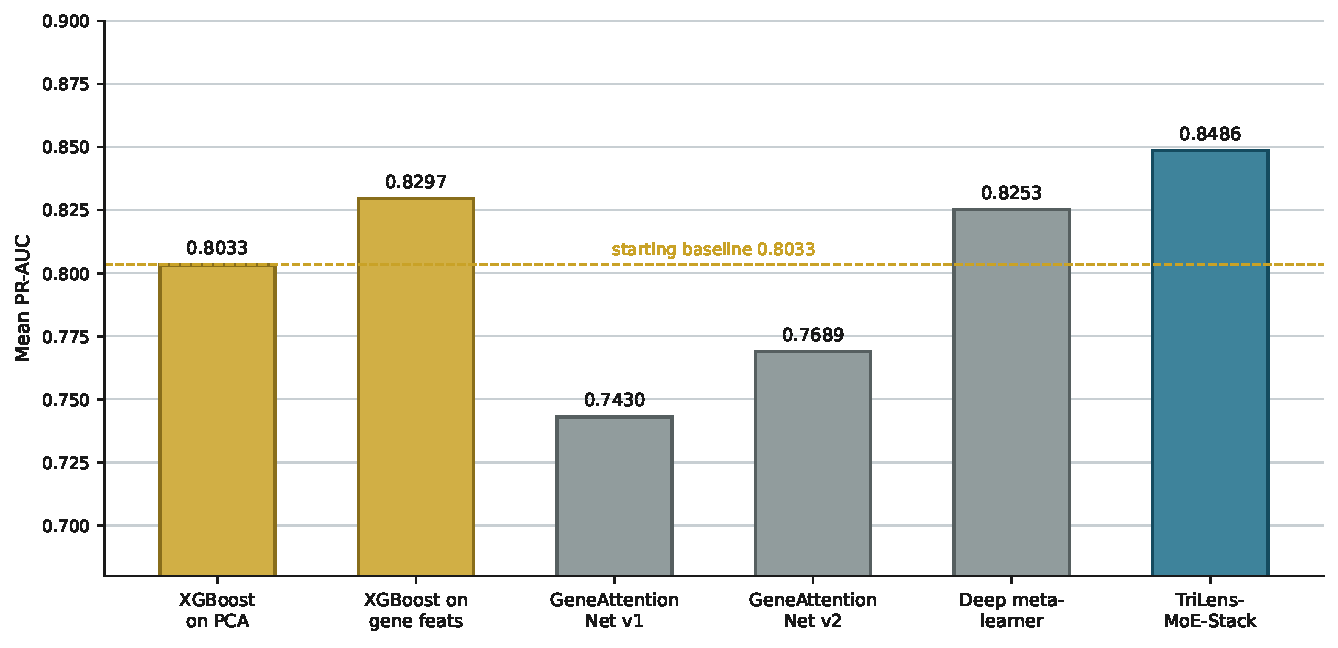
\includegraphics[width=\textwidth]{fig_progression.pdf}
\caption{The route to the final model, in the order the stages were built.}
\label{fig:progression}
\fignote{The two purely neural designs sit below the gradient-boosting baseline they
were meant to improve on, and the deeper meta-learner is worse than the simple one it
replaced. The vertical axis is truncated at 0.68 so that differences of a few
thousandths remain visible; no bar starts at zero.}
\end{figure}

The first true win came from features rather than models. Switching from PCA
components to gene-level features increased the score from 0.803 to 0.830 without
changing the learner at all, as aggregating variants per gene provided the model
with a biologically-meaningful input. Single neural models were disappointing:
GeneAttentionNet v1 only attained 0.743, worse than the plain XGBoost baseline,
and a second version only improved to 0.7689 after testing 7 design variants but
lost to XGBoost on all 7 antibiotics. It was the first clear indication we had
that purely neural approaches were not going to win here. At 0.8253, switching
from the logistic meta-learner to a deeper neural one made things worse. In fact,
taken as a whole, the table marks a ceiling: once the features were right,
none of our designs could go much beyond 0.85.

Because our neural lenses failed to outperform the classical learners, it would be
fair to ask us whether some other deep learning architecture would succeed.
Training TabNet, which is an architecture that targets tabular data, was done on
the same features with the same split, and Figure~\ref{fig:tabnet_vs_trilens} sets the
result beside the gradient-boosting baseline and our own model.

\begin{figure}[htb]
\centering
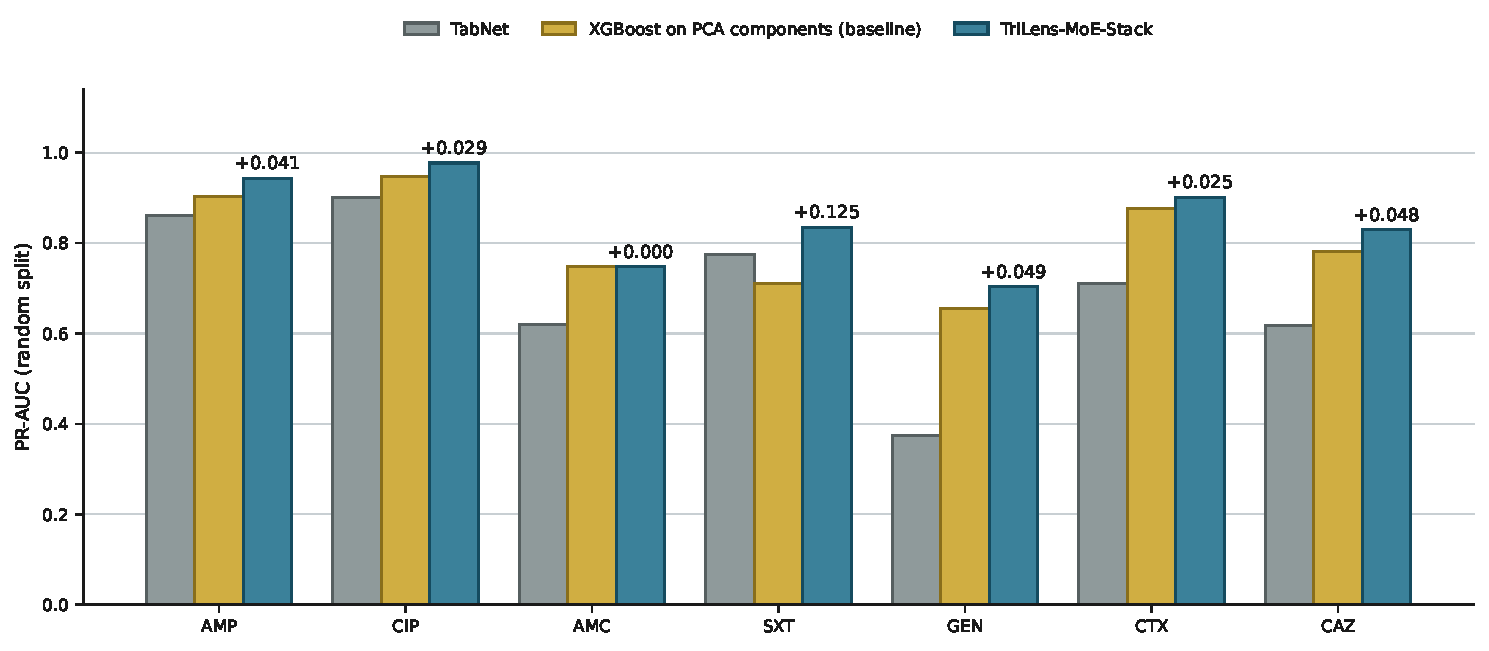
\includegraphics[width=\textwidth]{fig_tabnet_vs_trilens.pdf}
\caption{TabNet, the gradient-boosting baseline and TriLens-MoE-Stack, by antibiotic,
on the random split.}
\label{fig:tabnet_vs_trilens}
\fignote{The figure above each blue bar is the gain over the baseline, not over
TabNet.}
\end{figure}

The difference is large
and consistent. On each antibiotic individually, our model wins, on average by
0.154 (range, 0.061 on trimethoprim-sulfamethoxazole to 0.329 on gentamicin).
Consider gentamicin, the most clear-cut case; TabNet scored a mere 0.3751 on this
one when ours got 0.7037, and during training its validation score on that drug
swung between 0.58 and 0.80 from epoch to epoch and never settled. This does
not help establish the case of a general-purpose deep learning model for tabular
data alone, and both this comparison and the baseline ladder of
Table~\ref{tab:baselines} point in the same direction: it is the combination, not
the depth, that helps. The middle bar of each group is the gradient-boosting
baseline this project started from, and it tells a different story. That margin is
much smaller and far less even. It is widest on trimethoprim-sulfamethoxazole and
close to nothing on amoxicillin with clavulanic acid, where the baseline is
already almost as good as the finished model. A deep tabular model is not the
thing to beat here. The gradient-boosting baseline is.

\FloatBarrier
\subsection{The Lineage Holdout: Performance on Strains from Unseen Lineages}
\label{subsec:prevmatch}

The question posed in this subsection is more difficult: does the model
continue to work when it is presented with a strain it has never seen
before? The phylogroup-stratified split fails to do
it: it rearranges the information within eight large clusters, thus leaving a
strain and a close one on different sides, and its performance under it changes
little, between 0.849 and 0.853. This is not a test of unfamiliar strains, and
therefore could not have indicated a drop in any way.

The holdout which answers it makes use of the type of sequence of each strain, a
common designation of bacterial genetics according to which strains are clustered
by lineage. We successfully called a type of sequence to 6,487 of the 6,962
strains, or 93.2 per cent, with a total of 458 types, including a couple of giant
ones: sequence type 73 alone has 884 strains, or nearly one in every eight of the
samples. There were two rules prior to peeking at any outcome. Any strain whose
sequence type had no reliable sequence type was put into training and here, any
sequence type that comprised over five percent of the data was also put into
training, as a test set constructed using mostly a single clone would not be
testing generalisation. That condition was fulfilled by four types, namely, ST73,
ST131, ST95 and ST69. The other 454 sequences were assigned whole (not split),
using a fixed random seed such that no sequence type appears in more than one of
the training, validation and test sets.

The outcome was just the opposite. Mean performance plummets to 0.634 when they
are split by the lineage holdout, a decrease of over a fifth, and that is what the
phylogeny split had been unable to discover since it did not wipe any lineage off
training. Table~\ref{tab:mlst_per_ab} positions the three splits next to each
other.

\FloatBarrier
\begin{table}[htb]
\centering
\caption{Per-antibiotic PR-AUC under all three splits, with the drop measured from
the random split to the lineage holdout. Rows are ordered by that raw drop;
Figure~\ref{fig:lineage_drop} orders the same antibiotics by the
prevalence-corrected gap instead, which moves ciprofloxacin and
amoxicillin-clavulanate.}
\label{tab:mlst_per_ab}
\small
\begin{tabular}{|l|r|r|r|r|}
\hline
\textbf{Antibiotic} & \textbf{Random split} & \textbf{Phylogroup-strat.} & \textbf{Lineage holdout} & \textbf{Drop} \\ \hline
AMP & 0.9440 & 0.9338 & 0.9043 & $\mathbf{-0.040}$ \\ \hline
SXT & 0.8352 & 0.8373 & 0.7872 & $-0.048$ \\ \hline
CIP & 0.9773 & 0.9617 & 0.9118 & $-0.066$ \\ \hline
AMC & 0.7482 & 0.7963 & 0.4865 & $-0.262$ \\ \hline
CTX & 0.9019 & 0.8807 & 0.6073 & $-0.295$ \\ \hline
CAZ & 0.8299 & 0.8481 & 0.4930 & $-0.337$ \\ \hline
GEN & 0.7037 & 0.7136 & 0.2457 & $\mathbf{-0.458}$ \\ \hline
\textbf{Average} & \textbf{0.8486} & \textbf{0.8531} & \textbf{0.6337} & \\ \hline
\end{tabular}
\vspace{0.4em}

\noindent\footnotesize\textit{Note:} Ampicillin's drop of $-0.040$ is the smallest under the
lineage holdout and gentamicin's $-0.458$ the largest, the two-group pattern this chapter keeps
coming back to. Bold marks the extreme values in a column, best and worst alike.
\end{table}

\begin{figure}[htb]
  \centering
  \resizebox{\textwidth}{!}{\begin{tikzpicture}[x=1.95cm, y=7.0cm]

\foreach \y in {0,0.2,0.4,0.6,0.8,1.0}{
  \draw[black!20,line width=0.4pt] (0.45,\y) -- (8.15,\y);
  \node[anchor=east,font=\small,text=black] at (0.40,\y) {\y};
}

\draw[black,line width=0.9pt] (0.45,0) -- (8.15,0);
\draw[black,line width=0.9pt] (0.45,0) -- (0.45,1.06);
\node[rotate=90,anchor=south,font=\small,text=black] at (0.00,0.53) {PR-AUC};

\foreach \i/\ab/\rnd/\hold/\mat/\gap in {%
  1/AMP/0.9440/0.9043/0.9268/{-0.017},
  2/CIP/0.9773/0.9118/0.9471/{-0.030},
  3/SXT/0.8352/0.7872/0.8046/{-0.031},
  4/CTX/0.9019/0.6073/0.7260/{-0.176},
  5/CAZ/0.8299/0.4930/0.6431/{-0.187},
  6/AMC/0.7482/0.4865/0.5513/{-0.197},
  7/GEN/0.7037/0.2457/0.4594/{-0.244}}{
    \fill[bluefill]  (\i-0.335,0) rectangle (\i-0.135,\rnd);
    \draw[blueedge,line width=0.6pt] (\i-0.335,0) rectangle (\i-0.135,\rnd);
    \fill[redfill]   (\i-0.10,0) rectangle (\i+0.10,\hold);
    \draw[rededge,line width=0.6pt] (\i-0.10,0) rectangle (\i+0.10,\hold);
    \fill[greenfill] (\i+0.135,0) rectangle (\i+0.335,\mat);
    \draw[greenedge,line width=0.6pt] (\i+0.135,0) rectangle (\i+0.335,\mat);
    \node[anchor=north,font=\small,text=black] at (\i,-0.014) {\ab};
    \node[anchor=south,font=\scriptsize,text=black] at (\i,\rnd+0.014) {\gap};
}

\draw[black!55,dashed,line width=0.8pt] (3.5,0) -- (3.5,1.04);
\node[anchor=south,font=\scriptsize\itshape,text=black,align=center]
  at (2.0,1.04) {mechanism-driven\\(small corrected gap)};
\node[anchor=south,font=\scriptsize\itshape,text=black,align=center]
  at (5.3,1.04) {lineage-dependent\\(large corrected gap)};

\fill[white] (6.42,0.770) rectangle (8.14,1.010);
\draw[black!25,line width=0.5pt] (6.42,0.770) rectangle (8.14,1.010);

\fill[bluefill] (6.50,0.940) rectangle (6.68,0.978);
\draw[blueedge,line width=0.6pt] (6.50,0.940) rectangle (6.68,0.978);
\node[anchor=west,font=\scriptsize,text=black] at (6.74,0.959) {Random split};

\fill[redfill] (6.50,0.872) rectangle (6.68,0.910);
\draw[rededge,line width=0.6pt] (6.50,0.872) rectangle (6.68,0.910);
\node[anchor=west,font=\scriptsize,text=black] at (6.74,0.891) {Lineage holdout};

\fill[greenfill] (6.50,0.804) rectangle (6.68,0.842);
\draw[greenedge,line width=0.6pt] (6.50,0.804) rectangle (6.68,0.842);
\node[anchor=west,font=\scriptsize,text=black] at (6.74,0.823) {Prevalence-matched};

\end{tikzpicture}
}
  \caption{Random split, the lineage holdout as measured, and the same holdout
  resampled to the training prevalence.}
  \label{fig:lineage_drop}
  \fignote{Bars are ordered by the prevalence-corrected gap, which is printed above
  each group, so the order differs from Table~\ref{tab:mlst_per_ab}, which is ordered
  by the raw drop. Three antibiotics lose 0.017 to 0.031 once prevalence is corrected
  for and four lose 0.176 to 0.244, with nothing in between. The values behind this
  figure are in Table~\ref{tab:previnv}.}
\end{figure}

The trend is not anywhere near homogenous and Figure~\ref{fig:lineage_drop}
renders the split apparent: three antibiotics struggle to move, four fall
sharply. Ampicillin has a loss of only 0.040 and gentamicin has a loss of 0.458.
It is the same ranking as in Sections~\ref{sec:perfeval} and~\ref{subsec:layerabl},
only much more emphatic here, since this is the first time a lineage has been
removed as opposed to reshuffled. The third bar in each group takes the
prevalence effect out, and the rest of this section explains what that means.

\vspace{1em}

There are two objections to be met before all this can be credited. One is that a
failure to generalise is not the only way a drop this large can occur,
it can also be caused by near-duplicate strains. On this split zero of the
1{,}045 test strains had a close match in training, using the same
nearest-neighbour scan described in Section~\ref{sec:statanalysis}, which found
47 such strains on the random split. The middle column of the table demonstrates this for the
phylogroup-stratified split: four antibiotics outperform the random split
and none declines by more than 0.022, which is not the behaviour of a split
that truly withholds a lineage. The second
objection does need correcting for: the holdout downwardly shifts the test-set
resistance prevalence for each antibiotic by between 2.5 and 12.1 percentage
points; gentamicin has only 38 resistant strains left. That has to be
distinguished from the drop before the drop can be interpreted as a loss of
skill.

\vspace{1em}

An unskilled classifier has an expected PR-AUC equal to the prevalence of the
positive class. This means that the whole scale on which PR-AUC is judged
moves with prevalence. A test partition containing fewer resistant strains
will therefore score lower even if the model ranks the strains in the same
order as before. We refer to this as the no-skill baseline rather than a
floor, because a poor enough classifier can still score below it. The
opposite extreme is gentamicin, with only 38 resistant
in its holdout test set, a prevalence of 4.2 percent as compared to 14.6 percent
in training.

\vspace{1em}

We directly measured the size of this effect. We repeatedly subsampled the
susceptible strains in the holdout test set to obtain the same prevalence as the
training set and recomputed PR-AUC on the same saved predictions for each
antibiotic. No model was re-trained and no resistant strain was abandoned.
Table~\ref{tab:previnv} presents mean over 2{,}000 resampling rounds with 95 per
cent interval and ROC-AUC with no-skill value of 0.5 irrespective of prevalence.

\FloatBarrier
\begin{table}[htb]
\centering
\caption{The lineage holdout with the prevalence effect removed. The
prevalence-matched column resamples the holdout test set to the training
prevalence; the final column is the resulting gap against the random split.}
\label{tab:previnv}
\small
\setlength{\tabcolsep}{4pt}
\begin{tabular}{|l|>{\raggedleft\arraybackslash}p{1.7cm}|>{\raggedleft\arraybackslash}p{2.0cm}|>{\raggedleft\arraybackslash}p{3.4cm}|>{\raggedleft\arraybackslash}p{1.6cm}|>{\raggedleft\arraybackslash}p{1.6cm}|}
\hline
\textbf{Antibiotic} & \textbf{Random split} & \textbf{Holdout, as measured} & \textbf{Holdout, prevalence-matched} & \textbf{ROC-AUC} & \textbf{True gap} \\ \hline
AMP & 0.9440 & 0.9043 & 0.9268 [0.918, 0.938] & 0.9257 & $\mathbf{-0.017}$ \\ \hline
CIP & 0.9773 & 0.9118 & 0.9471 [0.926, 0.967] & 0.9739 & $-0.030$ \\ \hline
SXT & 0.8352 & 0.7872 & 0.8046 [0.792, 0.823] & 0.9038 & $-0.031$ \\ \hline
CTX & 0.9019 & 0.6073 & 0.7260 [0.687, 0.766] & 0.8838 & $-0.176$ \\ \hline
CAZ & 0.8299 & 0.4930 & 0.6431 [0.600, 0.679] & 0.7878 & $-0.187$ \\ \hline
AMC & 0.7482 & 0.4865 & 0.5513 [0.529, 0.584] & 0.6894 & $-0.197$ \\ \hline
GEN & 0.7037 & 0.2457 & 0.4594 [0.398, 0.511] & 0.7426 & $\mathbf{-0.244}$ \\ \hline
\textbf{Average} & \textbf{0.8486} & \textbf{0.6337} & \textbf{0.7226} & \textbf{0.8439} & $\mathbf{-0.126}$ \\ \hline
\end{tabular}
\vspace{0.4em}

\noindent\footnotesize\textit{Note:} Once prevalence is corrected for, ampicillin's true gap is
$-0.017$, near nothing, against gentamicin's $-0.244$; the average true gap of $-0.126$ is still
well below the raw 0.215 gap the uncorrected numbers would suggest. Bold marks the extreme
values in a column, best and worst alike.
\end{table}

Only about two-fifths of the headline drop is a prevalence effect. Average
PR-AUC falls from 0.8486 (random split) to 0.7226 when prevalence is fixed, a
difference of 0.126, instead of 0.6337, a difference of 0.215, as the raw
holdout values would have indicated. As its own ROC-AUC of 0.7426 already
indicated, gentamicin is the one that most recovers, and its PR-AUC increases
from 0.2457 to 0.4594: the model had not ceased to rank resistant strains
above susceptible strains, it has merely been forced to do so on a test set
where only one in twenty-four strains is resistant.

Adjusting the prevalence does not remove the discovery, instead it clarifies
it. The seven antibiotics remain divided into the same two categories, but
even more distant relative to each other. Ampicillin, ciprofloxacin and
trimethoprim-sulfamethoxazole have a loss of 0.017 to 0.031 in PR-AUC, which
is near nothing, and cefotaxime, ceftazidime, amoxicillin-clavulanate and
gentamicin have a loss of 0.176 to 0.244, and no antibiotic is in between. A
model that had merely deteriorated on a more challenging set of tests would
exhibit an even distribution of losses among all seven drugs rather than this
two group divide. Amoxicillin-clavulanate is the cleanest: its prevalence
changes only by 5.9 points, thus it recovers the least of the four hard drugs
(a PR-AUC increase of 0.065, compared to gentamicin's 0.214) and also has the
lowest ROC-AUC of all seven, at 0.6894, so the least of its loss can be
attributed to prevalence at all.

Two caveats apply to this table. First, gentamicin's prevalence-matched
interval is wide, [0.398, 0.511], because it is anchored by only 38 resistant
strains, so its exact value should be read with caution even though its
direction is clear. Second, the holdout prevalence used for matching is the
\textit{training} prevalence, which is slightly higher than the random-split
test set's prevalence; this makes the comparison somewhat generous to the
holdout, so the true gap may be a little larger than the 0.126 reported
above.

\vspace{1em}

What the holdout costs in clinical terms is the next question.
Section~\ref{sec:perfeval} reported clinical error rates on the random split. Of
greater interest is what happens to the errors that get to a patient if the
strain is from an unfamiliar lineage. Table~\ref{tab:holdoutclin} does, using the
same saved predictions and the same fixed threshold of 0.5, and
Figure~\ref{fig:clinical_heatmap} does the same with the numbers arranged by
severity.

\FloatBarrier
\begin{table}[htb]
\centering
\caption{Clinical error rates under the lineage holdout against the random split,
at a threshold of 0.5. Being within-class ratios, VME and ME are unaffected by the
prevalence shift. Rows are ordered by holdout VME, the same order as
Figure~\ref{fig:clinical_heatmap}.}
\label{tab:holdoutclin}
\small
\setlength{\tabcolsep}{4pt}
\resizebox{\textwidth}{!}{%
\begin{tabular}{|l|>{\raggedleft\arraybackslash}p{1.7cm}|>{\raggedleft\arraybackslash}p{1.3cm}|>{\raggedleft\arraybackslash}p{1.3cm}|>{\raggedleft\arraybackslash}p{1.5cm}|>{\raggedleft\arraybackslash}p{1.3cm}|>{\raggedleft\arraybackslash}p{1.3cm}|>{\raggedleft\arraybackslash}p{1.3cm}|>{\raggedleft\arraybackslash}p{1.3cm}|}
\hline
\textbf{Antibiotic} & \textbf{Resistant in test} & \textbf{VME random} & \textbf{VME holdout} & \textbf{Increase} & \textbf{ME random} & \textbf{ME holdout} & \textbf{CA random} & \textbf{CA holdout} \\ \hline
CIP & 132 & 0.086 & 0.114 & $+0.028$ & 0.015 & 0.006 & 0.969 & 0.978 \\ \hline
AMP & 300 & 0.109 & 0.160 & $+0.051$ & 0.104 & 0.095 & 0.893 & 0.877 \\ \hline
SXT & 142 & 0.236 & 0.310 & $+0.074$ & 0.080 & 0.072 & 0.871 & 0.863 \\ \hline
AMC & 145 & 0.394 & 0.710 & $+0.316$ & 0.108 & 0.076 & 0.804 & 0.754 \\ \hline
CAZ & 43  & 0.291 & \textbf{0.837} & $+0.546$ & 0.033 & 0.001 & 0.936 & 0.959 \\ \hline
GEN & 38  & 0.436 & \textbf{0.868} & $+0.432$ & 0.023 & 0.002 & 0.934 & 0.962 \\ \hline
CTX & 71  & 0.190 & \textbf{0.915} & $+0.725$ & 0.026 & 0.001 & 0.953 & 0.918 \\ \hline
\textbf{Mean} & & \textbf{0.249} & \textbf{0.559} & $\mathbf{+0.310}$ & \textbf{0.056} & \textbf{0.036} & & \\ \hline
\end{tabular}
}
\vspace{0.4em}

\noindent\footnotesize\textit{Note:} Gentamicin (0.868), ceftazidime (0.837) and cefotaxime
(0.915) all have a holdout VME above 0.83, meaning the model has effectively stopped finding
resistance for these three; the mean row averages across all seven.
\end{table}

\begin{figure}[htb]
\centering
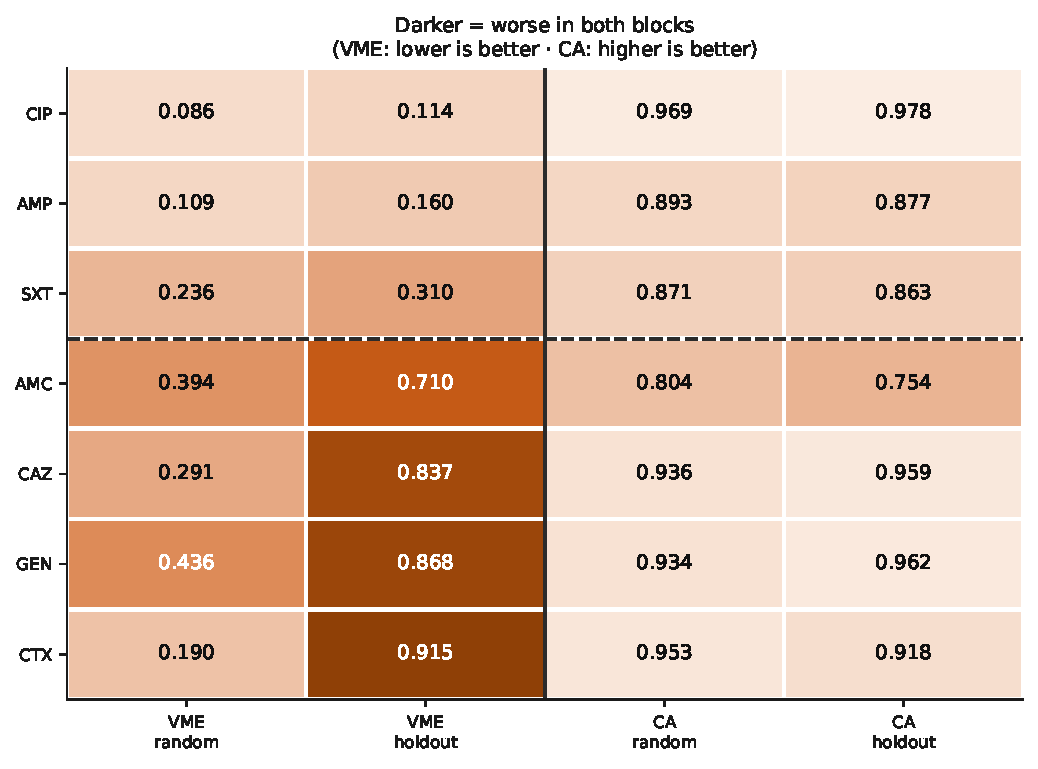
\includegraphics[width=\textwidth]{fig_clinical_heatmap.pdf}
\caption{Very major error rate and categorical agreement, random split against
lineage holdout.}
\label{fig:clinical_heatmap}
\fignote{Both blocks use a single scale on which a darker cell is the worse result.
The categorical-agreement columns are shaded by $1-\mathrm{CA}$ so that the
convention holds throughout. Drugs are ordered by holdout very major error rate; the
dashed line marks the split between the two groups.}
\end{figure}

The average very major error rate increases from 0.249 to 0.559 and for three
antibiotics, the model has completely ceased to detect resistance. It detects
6 of the 71 cefotaxime-resistant strains, 5 of the 38
gentamicin-resistant strains and 7 of the 43 ceftazidime-resistant strains, with a
major error rate of 0.001 or 0.002 for each group. That combination is the
hallmark of a classifier that has collapsed onto the
majority class: it hardly ever makes a resistant prediction, so it hardly ever
makes such predictions wrongly. These numbers are more difficult to dispute
than the PR-AUC values above since VME and ME are calculated within a class and
stay fixed as the class mix varies. Prevalence-matching resamples only
susceptible strains, and very major error rate is considered to be all in the
resistant category, thus cannot be resampled. Clinical deterioration here
therefore has no prevalence component, and requires no correction before it can
be believed.

The categorical agreement column demonstrates why accuracy does not drive this
research. Three antibiotics show equal or higher categorical agreement in the
holdout than in the random split, and for the other four the reduction in
agreement is much smaller than the total collapse in clinical safety alongside
it. Gentamicin increases from 0.934 to 0.962 while very major error rate doubles
to 0.868; ceftazidime from 0.936 to 0.959, missing 36 of the 43 resistant
strains; cefotaxime changes by just 0.035 but its very major error rate rises from
0.190 to 0.915. By the measure a machine learning paper would use to report
results, this model looks better or nearly as good, on unseen lineages; by the
measure a clinician would use, it became unusable.

This is the third analysis to produce the same grouping. They are the same three
with the same saved predictions and test set, therefore they are complementary
views but measure different aspects of those predictions. The three antibiotics
with negligible loss in PR-AUC gain between 0.028 and 0.074 in very major error
rate, and the four with a significant loss have a gain of 0.316 to 0.725. The
order within the second group changes, as cefotaxime is worst in this group
whereas gentamicin was worst using PR-AUC, the rank within the groups is not to be
overly read, but the grouping, which is based on the drug's performance in the
corresponding group, does not change across all three analyses.

The holdout also allows us to redo the component analysis of
Section~\ref{subsec:layerabl} in more difficult conditions, and
Table~\ref{tab:mlst_components} shows that the outcome alters the previous
picture.

\FloatBarrier
\begin{table}[htb]
\centering
\caption{Average PR-AUC of each component of the model, under the lineage
holdout.}
\label{tab:mlst_components}
\small
\begin{tabular}{|l|r|}
\hline
\textbf{Component} & \textbf{Avg PR-AUC} \\ \hline
TriLens neural arm alone (lenses with gate) & 0.472 \\ \hline
Five classical learners alone & \textbf{0.628} \\ \hline
Full hybrid model & \textbf{0.634} \\ \hline
\end{tabular}
\vspace{0.4em}

\noindent\footnotesize\textit{Note:} The classical learners alone reach 0.628, close to the full
hybrid model's 0.634 under this harder split, meaning the neural lenses add almost nothing here.
The 0.634 in the last row is the 0.6337 reported to four decimal places in
Table~\ref{tab:mlst_per_ab}. The 0.628 in the middle row is the five base
learners \emph{stacked}, and is a different quantity from the 0.6299 of
Table~\ref{tab:vsraw}, which is the single strongest learner on its own: under
this split the stacking layer recovers slightly less than its own best member
already had.
\end{table}

The neural arm alone, that is the three lenses with the gate, scored 0.781 on the
random split (Section~\ref{subsec:layerabl}). It plummets to 0.472 here, when tested on truly
unseen lineages; this represented a much larger decline compared to what the
classical learners achieve on their own (0.628), nearly matching the full hybrid
model (0.634). The classical learners do nearly all of the work under a true test
of generalisation and the neural lenses add almost nothing. It is a stronger
form of what Section~\ref{subsec:layerabl} already indicated: the gap between
the two arms is 0.156, and the fused model only
recovers 0.006 of it. But this was not a case where some other deep learning
design would have generalised better; TabNet reran on this split averages 0.326,
worse than our neural lenses on their own and well below the classical learners.
Gradient-boosted trees on gene-level features are the best method we identified
on this dataset and under this type of test.

\vspace{1em}

The downside on unseen lineages gives one an obvious next question: does it work
at all on a different set of strains? The two datasets do not have a shared
feature vector as Arcadia uses the pan-genome reference with 535{,}000 variant
positions and Giessen uses a single reference with approximately 60{,}000
variant positions. We rather trained the classical stacking part of the pipeline
on Giessen with the same protocol and hyperparameters. The three neural lenses
require feature shapes only the pan-genome view can provide and thus are not
included in this comparison; and four antibiotics are in common to both
collections. The Giessen collection is summarised in Figure~\ref{fig:giessen_overview}
prior to the reporting of how well the classical stack transfers to it in
Table~\ref{tab:giessen_transfer}, with Figure~\ref{fig:giessen_retention} setting the
rebuilt scores beside their Arcadia counterparts.

\FloatBarrier
\begin{figure}[htb]
\centering
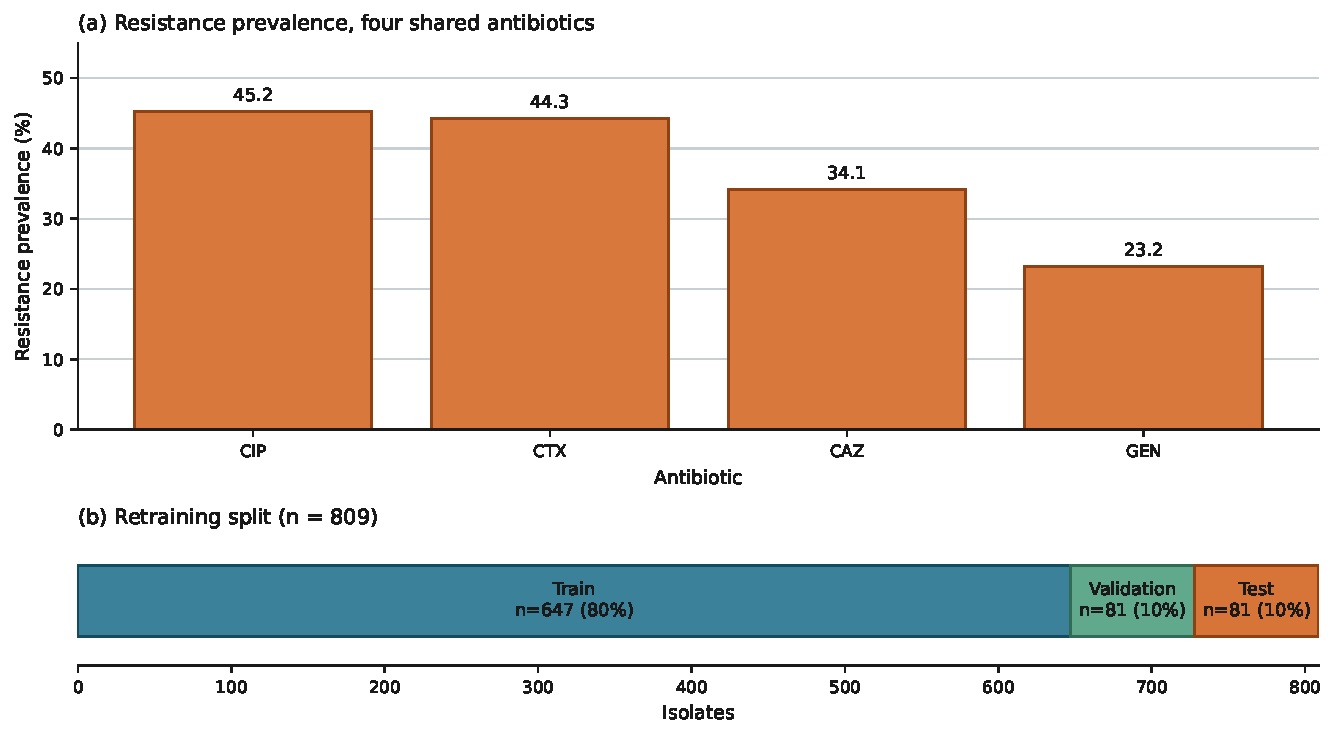
\includegraphics[width=\textwidth]{fig_giessen_overview.pdf}
\caption{The Giessen set: resistance prevalence and the retraining split.}
\label{fig:giessen_overview}
\fignote{\textbf{(a)} Resistance prevalence for the four shared antibiotics.
\textbf{(b)} The 647/81/81 retraining split (n = 809). Every isolate here carries a
label for all four antibiotics, so nothing is missing.}
\end{figure}

\begin{table}[htb]
\centering
\caption{The classical stacking half of the pipeline, trained independently on a
second collection. Neither column is the full TriLens model.}
\label{tab:giessen_transfer}
\small
\begin{tabular}{|l|r|r|r|}
\hline
\textbf{Antibiotic} & \textbf{Arcadia} & \textbf{Giessen} & \textbf{Retention} \\ \hline
CIP & 0.9773 & 0.9868 & \textbf{101.0\%} \\ \hline
CAZ & 0.8299 & 0.7775 & 93.7\% \\ \hline
CTX & 0.9019 & 0.7876 & 87.3\% \\ \hline
GEN & 0.7037 & 0.5480 & \textbf{77.9\%} \\ \hline
\textbf{Average} & \textbf{0.8532} & \textbf{0.7750} & \textbf{90.0\%} \\ \hline
\end{tabular}
\vspace{0.4em}

\noindent\footnotesize\textit{Note:} Ciprofloxacin's apparent 101.0\% retention is the highest in
the table and gentamicin's 77.9\% the lowest, matching the ordering seen under the lineage
holdout. As the text below explains, these retention figures are inflated by Giessen's higher
prevalence rather than by genuinely better performance. Bold marks the extreme values in a
column, best and worst alike.
\end{table}

\begin{figure}[htb]
\centering
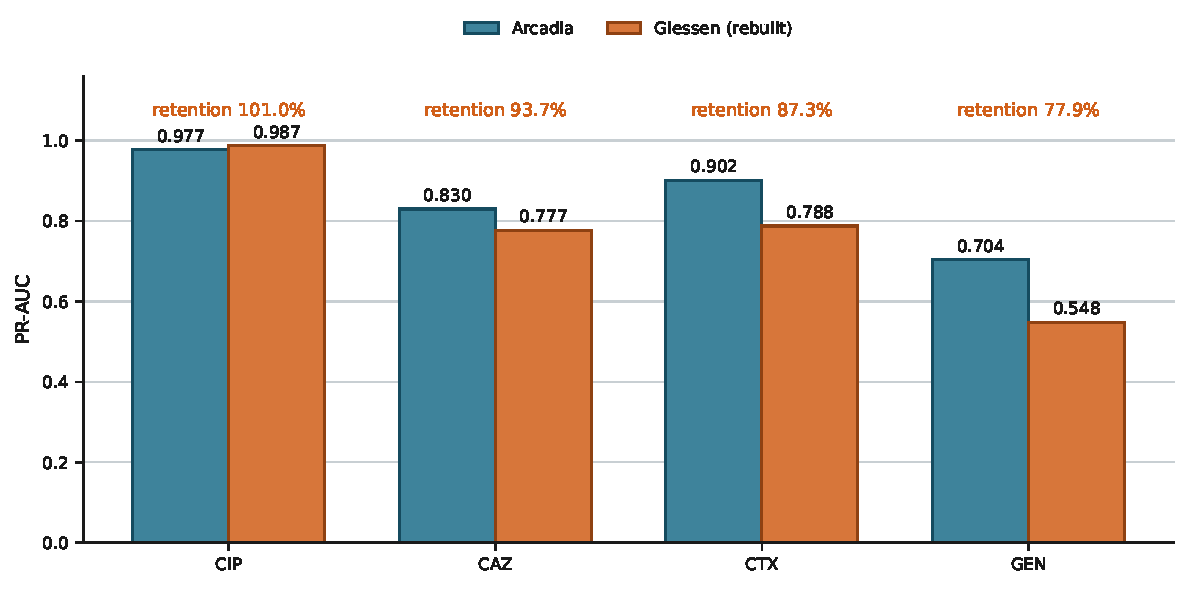
\includegraphics[width=\textwidth]{fig_giessen_retention.pdf}
\caption{The classical stack rebuilt on the Giessen collection, against its Arcadia
scores.}
\label{fig:giessen_retention}
\fignote{Ciprofloxacin transfers almost intact while gentamicin retains least, the
same ordering the lineage holdout produces. The retention figures are inflated by
Giessen's higher prevalence, as the text below explains.}
\end{figure}

The approach keeps about 90\% of its performance on a genomically different
collection. It is not zero-shot transfer, in that the model was retrained; what
it demonstrates is that our design decisions are not optimized to the specifics
of a single dataset.

\vspace{1em}

There is one caveat here, the same one this chapter raises so many times
elsewhere. Section~\ref{subsec:prevmatch} holds that PR-AUC cannot be compared
across partitions with differing prevalence, and the two collections differ
significantly in prevalence. In Arcadia, the resistance of ciprofloxacin
stands at 0.228 as compared to 0.452 in Giessen. Cefotaxime is 0.152 resistant
in Arcadia as compared to 0.443 in Giessen. In Arcadia, ceftazidime is 0.131
resistant against 0.341 in Giessen. Gentamicin has a resistance of 0.118 in
Arcadia compared to 0.232 in Giessen. In Giessen, every drug's no-skill
baseline is about twice to three times Arcadia's, before the model is
credited with any skill at all. So the
retention percentages are misleading by this difference in baselines, not by any
actual improvement, and perhaps the most transparent example is ciprofloxacin
whose apparent 101\% indicates that the model is marginally better on Giessen,
but what really happened is that Giessen made the task marginally easier. The
bias cannot be eradicated, because prevalence-matching would require both
collections to be resampled to an identical reference, and the 81-strain Giessen
test partition is too small to survive that exercise. The weaker argument is the
one we will justify from this table: that the recipe reconstructs and does not
fall apart, not that performance is maintained to within ten percent of its
original extent. The interesting part is the per-antibiotic pattern.
Ciprofloxacin retains most of its performance and gentamicin only 77.9\% of its
own, the same order as under the lineage holdout, though reached by an entirely
different route.

\FloatBarrier
\subsection{Comparison with Published Work on the Same Dataset}
\label{subsec:published}

The group that originally released our dataset subsequently published its own
analysis of the same strains \cite{york2025amr}. That gives us a rare chance
to independently audit our results against theirs. The two studies count different
things, so cannot be directly compared with the numbers they produce, nor ours.
Arcadia applied a Bayesian sparse linear mixed model fit to the complete dataset
and reported \emph{heritability}, a measure of the proportion of the variance in
a trait that can be attributed to genetic variation among individuals, while we
trained a classifier and reported PR-AUC (area under the precision-recall curve)
on an independent test set, a measure of the classifier's ability to predict
strains it has not previously seen; a trait may be highly heritable but, at the
same time, difficult to predict on new samples. They also investigated three
antibiotics against our seven and 7{,}043 strains as opposed to our 6{,}962.
What we can compare are the results, and there the agreement is remarkable
despite very different approaches. Table~\ref{tab:arcadia} sets the two accounts
side by side.

\begin{table}[htb]
\centering
\caption{Our findings against the published analysis of the same dataset. The two
studies report different measures, so only the biological conclusions are
compared.}
\label{tab:arcadia}
\small
\begin{tabular}{|>{\raggedright\arraybackslash}p{3.3cm}|>{\raggedright\arraybackslash}p{5.3cm}|>{\raggedright\arraybackslash}p{5.3cm}|}
\hline
\textbf{Topic} & \textbf{Arcadia analysis \cite{york2025amr}} & \textbf{This work} \\ \hline
Driver of ciprofloxacin resistance &
Three linked mutations: two in \textit{gyrA} and one in \textit{parC} &
\textbf{\textit{gyrA} and \textit{parC} appear among our top marker genes} \\ \hline
Driver of ampicillin resistance &
Plasmid and transposon fragments, led by a TEM-1 beta-lactamase &
A beta-lactamase gene appears among our markers \\ \hline
Driver of trimethoprim-sulfamethoxazole resistance &
No interpretable resistance locus could be identified &
No resistance gene was found for this antibiotic either \\ \hline
Reason some resistance genes are hard to find &
The pan-genome is fragmented, so plasmid-borne genes assemble poorly &
The same explanation fits our weak results for GEN and AMC \\ \hline
\end{tabular}
\vspace{0.4em}

\noindent\footnotesize\textit{Note:} The ciprofloxacin row is the strongest agreement in the
table: an independent team's mutation-level finding and our model's gene-level finding point to
the same two genes, \textit{gyrA} and \textit{parC}.
\end{table}

There are three rows that should be commented on. Our ciprofloxacin match is most
powerful: Arcadia had discovered three mutations each, at distinct locations in
\textit{gyrA} and \textit{parC}, whereas our model, which never received that
information, discovered the two genes by itself based on SHAP values on the
classical learners. The same outcome of trimethoprim-sulfamethoxazole is
interesting due to the opposite reason. Arcadia could not associate their best
markers with any known resistance mechanism and neither could we; they observed
that its best markers indicated aminoglycoside-related proteins, which have
nothing to do with this drug, and took on the hypothesis that the actual
resistance gene is located on a poorly assembled fragment of a plasmid on which
its best markers just happen to be situated. There was no other reasonable
explanation and it is heartening that, a specialist team also arrived at the
identical dead-end. Of particular importance to our discussion is the fragmented
pan-genome point, which, as Section~\ref{sec:discussion} indicates, is part of
the reason that gentamicin and amoxicillin-clavulanate do not work well, namely,
the fact that their resistance genes are carried on plasmids and transposons that
are not cleanly represented here. Arcadia came up with the same conclusion on a
different axis on their own and this gives us greater assurance that it must be
in the representation of data and not in our model.

There is one other number to discuss. The heritability values estimated by
Arcadia showed that the genetic markers in this dataset explain nearly all of the
variation between resistant and susceptible strains: 0.99 for ciprofloxacin, 0.95
for ampicillin and 0.94 for trimethoprim-sulfamethoxazole. The same three
antibiotics with the same values of PR-AUC on the random-split test set were 0.9773,
0.9440 and 0.8352; thus, ciprofloxacin is not far off what the heritability
suggests is possible, while trimethoprim-sulfamethoxazole is clearly behind.
Although the two sets of numbers are not directly comparable, the pattern is
informative: if the signal is nearly fully present in the markers, that limit of
$\sim$0.85 that all models in Table~\ref{tab:progression} reached is unlikely to be a
biological limit and more likely a limit of how the features are built. As stated
in Section~\ref{subsec:layerabl}, increased model complexity adds little and the
heritability estimates indicate the same trend from the other side. The missing
performance is not in a larger network, but in a better assembly, where the genes
of the plasmid and the transposon are no longer broken up and can be represented
as a complete gene.

\FloatBarrier
\subsection{Comparing Two Collections: The Cause of the Convolutional Network's Failure}
\label{subsec:cnnfail}

This section returns to the open question left by Section~\ref{subsec:ownprep}. Our initial
experiments with the 1D CNN were not successful, which led us to propose that the issue was
structural rather than a matter of tuning. A convolutional network learns local patterns from
adjacent positions, so if it is really learning from local structure, scrambling the order of the
input columns should destroy its performance, and leave it unchanged if the order never mattered.
The naive 1D CNN averaged 0.4826 on Arcadia against 0.6889 on Giessen, a difference of 0.2063,
but that gap proves nothing on its own, since the two collections differ in prevalence, labelling
standard and size. The shuffle test settles it by comparing each collection against itself.
Rerunning ciprofloxacin with the SNP columns shuffled, the two behaved in opposite ways: Giessen
declined from 0.8635 to 0.5411, a loss of 0.322, while Arcadia moved from 0.7473 to 0.7957 and so
gained a little. Where destroying the order raises the score, the model was not using order in the
first place. Table~\ref{tab:locality} sets out both halves of the test.

\begin{table}[htb]
\centering
\caption{The locality test. Panel (a) is the naive one-dimensional CNN trained
separately on each collection; panel (b) reruns ciprofloxacin with the SNP column
order permuted, a separate retraining run, which is why its ordered Giessen score
differs slightly from panel (a). All values are test PR-AUC, 95 per cent bootstrap
intervals in brackets.}
\label{tab:locality}
\small
\begin{tabular}{|l|c|c|r|}
\hline
\multicolumn{4}{|l|}{\textbf{(a) Naive 1D CNN, per antibiotic}} \\ \hline
\textbf{Antibiotic} & \textbf{Arcadia} & \textbf{Giessen} & \textbf{Gap} \\
                    & \textit{(pan-genome)} & \textit{(single reference)} & \\ \hline
CIP & 0.7473 & 0.8559 & $+0.109$ \\ \hline
CTX & 0.5107 & 0.8343 & $+0.324$ \\ \hline
CAZ & 0.3802 & 0.7535 & $+0.373$ \\ \hline
GEN & 0.2921 & 0.3117 & $+0.020$ \\ \hline
\textbf{Average} & \textbf{0.4826} & \textbf{0.6889} & $\mathbf{+0.206}$ \\ \hline
\end{tabular}

\vspace{1em}

\begin{tabular}{|l|c|c|r|}
\hline
\multicolumn{4}{|l|}{\textbf{(b) Ciprofloxacin with the SNP column order shuffled}} \\ \hline
\textbf{Collection} & \textbf{Ordered} & \textbf{Shuffled} & \textbf{Effect} \\ \hline
Giessen \textit{(single reference)} & 0.8635 & 0.5411 & $\mathbf{-0.322}$ \\
                                    & \footnotesize[0.781, 0.928]
                                    & \footnotesize[0.416, 0.668] & \\ \hline
Arcadia \textit{(pan-genome)}       & 0.7473 & 0.7957 & $+0.048$ \\
                                    & \footnotesize[0.682, 0.809]
                                    & \footnotesize[0.745, 0.843] & \\ \hline
\end{tabular}
\vspace{0.4em}

\noindent\footnotesize\textit{Note:} On Giessen the ordered and shuffled intervals do
not overlap and the shuffled model's MCC falls from 0.469 to 0.000, collapsing to
calling every strain resistant. On Arcadia the intervals overlap and the point estimate
moves \emph{upwards}, so there was no positional signal to destroy. That asymmetry is
the evidence for confining convolution to gene blocks.
\end{table}

The asymmetry can be explained by the way the two datasets are constructed. Giessen maps all strains
to one reference genome, so column 100 and column 101 really are adjacent locations on the same
chromosome. Arcadia employs a pan-genome reassembling a large number of strains, so two adjacent
columns may contain different contigs, different genes, or even different portions of the accessory
genome altogether, and there is no local structure to be sought. Lens A therefore convolves only
within each gene block, where positions are genuinely adjacent, and pools across genes with attention.

\FloatBarrier
\section{Discussion}
\label{sec:discussion}

The above results lead to a question which transcends model comparison. We find our model
reasonably predictive of resistance on familiar strains but the question of greater interest is
what it is actually learning to make such predictions, and how much of that survives on strains it
has never seen.

\FloatBarrier
\subsection{The Genes the Model Relies On}
\label{subsec:attnfix}

We obtained the most impactful genes based on two sources: the weights of attention within the
three neural lenses, and SHAP values obtained with the five classical base learners. This provided
1{,}138 marker genes in total which covered all antibiotics. Their prokka locus tags alone do not
provide us with any information, so we aligned them with the eggNOG functional annotation released
with the Arcadia dataset. We were successful in annotating 889 of the 1{,}138 markers, or 78.1\%,
with the others having no corresponding match and indicating them as not annotated instead of
making a best guess. Eight of the annotated markers were known genes involved in antimicrobial
resistance: gyrA, parC, the two target genes where point mutations result in fluoroquinolone
resistance; emrB, mdtC, mdtD, mdtO and cusA, which are parts of multidrug efflux pumps, and one
additional gene annotated as a beta-lactamase.

The genuine result is in finding gyrA and parC and it is more significant following the lineage
holdout than ever. These are the textbook objectives of ciprofloxacin resistance and ciprofloxacin
was the very antibiotic that did not succumb to the holdout most, dropping only 0.030 when
prevalence is held constant, as compared to other antibiotics that dropped up to 0.244. A model
based on an actual, conceptually clear mutation should be transferred to a new lineage and that is
what we observe. One detail, though, is more important than the list of genes. The eight resistance genes were all the
result of the SHAP analysis of the classical learners. None was a result of attention weights of
the three neural lenses, although, 420 out of the 1{,}138 markers were selected out of those
lenses.

\vspace{1em}

Two things besides a real failure could bring about that zero, and we tested each of them. The first is annotation coverage, as an eggNOG file lacks a gene and there is no
way to identify it as a resistance gene no matter how significant the model considered it to be.
The two of three lenses are eliminated by coverage: each of 140 markers contained in the
Cross-Antibiotic Context Module was annotated, and 97.9\% of markers in the Motif Pattern Encoder,
but neither generated a single resistance gene. The weaker case is the Gene Feature Attention
Module at 61.4\%, which is important as it is the lens the gate is most dependent on, thus the
view that our model believes is best will be the one that we can reasonably interpret least. The
second option is that twenty genes per lens per drug is too small a window and we did the
annotation in the top 100 genes five times, increasing coverage to 79.3\%. It also did not
reproduce any resistance gene, hence it is not an artefact of the position at which the list was
broken as well.

Another measurement can be used to explain why. The variant sweep that followed the final lens
design concentrated focus on the 5{,}000 selected genes instead of the entire catalogue of
32{,}441 genes, thus the maximum attainable entropy there was $\ln 5{,}000 \approx 8.52$, not the
$\ln 32{,}441 \approx 10.39$ of the full set. Compared against this lower ceiling, attention
entropy remains at 8.51 for trimethoprim-sulfamethoxazole, effectively at ceiling, and above 7.79
for amoxicillin-clavulanate, gentamicin, cefotaxime and ceftazidime, still at or within ten percent
of it. When the attention mass of the five drugs is at the most not even one percent of the total
mass, in any case, and when ninety percent of it is distributed amongst two or four thousand
genes, the pooling layer has virtually broken down into a mere mean. Only ampicillin and
ciprofloxacin exhibit real concentration, with entropies 5.34 and 5.46 with just under twenty
genes exceeding one percent each, and we by no means attribute biology to even that, since another
pooling function tested in a separate sweep concentrated on another group of drugs, indicating the
pattern follows the architecture and not the resistance mechanism.

\vspace{1em}

What it does focus on is still informative. Each gene in the pan genome has a locus
tag that indicates which of the assemblies the gene was called from, providing an inexpensive
method to determine which of the attended genes are sampled or from across the pan genome. For the
Gene Feature Attention Module they are not: for each of the 7 antibiotics, the top genes by this
module were concentrated in a single assembly between 12 times that assembly's fraction in the
catalogue and 23 times: median was 16.4. Those counts are less informative because they represent a
small number of genes per antibiotic, only genes with an assembly tag can be counted and that
counts less than a dozen genes in total, so we read the ratio more as an indicator of the direction
of the lens than as a formal test.

An obvious objection is that this is simply an artefact of how pan-genome clusters are named, as
each cluster takes the tag of whichever assembly represented it, and a well represented assembly
would then swamp any list by arithmetic. There are two reasons why not to think so. The assembly
the lens focuses on provides merely 3.3\% of the catalogue, therefore abundance cannot account
for a sixteen-fold preference. And the other two lenses do only just what the artefact explanation
would predict: both focus on the \textit{most} populous tag they are reading, at an enrichment of
only 1.6 to 2.1, so that we do not report them as a discovery. The natural interpretation of that
enrichment, then, is that the lens has learnt a lineage fingerprint,
i.e. genes that are expected to be transmitted along a branch of the population will indeed be
transmitted along the same branch of the population. We attempted to test this rather than simply
assuming it was right. The reading does not hold: as Table~\ref{tab:umark} later in this section
shows, the attended genes are \emph{less} lineage-determined than a randomly chosen gene, not
more.

\vspace{1em}

These above are what attention still cannot do. They are, however, much better than the results
obtained via a direct application of gated attention pooling on this input, and this difference is
one of the design contributions of this work: it is the only area where we changed the mechanism
itself rather than the data it reads from. Section~\ref{subsec:lensB} and
Equations~\eqref{eq:expertB_ctx}--\eqref{eq:expertB_score} set out the argument in full: on a
presence-and-absence vector the standard gated-attention score becomes simply that gene's
embedding, and is thus identical for all strains that carry that gene, and conditioning it on the
mean embedding of the genes the strain actually carries restores per-sample behaviour. As this
reasoning predicts a behaviour, we evaluated it in an ablation, training the model in both
directions using the same seeds, folds, splits and hyperparameters, changing only this single
term. Table~\ref{tab:attnfix} reports the effect.

{\small
\setlength{\tabcolsep}{4pt}
\setlength{\LTpost}{0pt}
\begin{longtable}{|>{\raggedright\arraybackslash}p{7.6cm}|>{\centering\arraybackslash}p{2.0cm}|>{\centering\arraybackslash}p{2.2cm}|>{\centering\arraybackslash}p{1.9cm}|}
\caption{Ablation of strain conditioning in the Gene Feature Attention Module.
Only this term differs; the second column is the delivered model.}
\label{tab:attnfix}\\
\hline
\textbf{Measure} & \textbf{Standard} & \textbf{Strain-cond. (delivered)} & \textbf{Change} \\
\hline
\endfirsthead
\hline
\textbf{Measure} & \textbf{Standard} & \textbf{Strain-cond. (delivered)} & \textbf{Change} \\
\hline
\endhead
\hline
\multicolumn{4}{r}{\footnotesize\textit{Continued on the next page}}\\
\endfoot
\hline
\endlastfoot
\multicolumn{4}{|l|}{\textit{Predictive performance}} \\ \hline
Random split, full stack & 0.8462 & 0.8486 & $+0.0024$ \\ \hline
Phylogroup-stratified split & 0.8519 & 0.8531 & $+0.0012$ \\ \hline
Lineage holdout, full stack & 0.6300 & 0.6337 & $+0.0037$ \\ \hline
Lineage holdout, classical learners only & 0.628 & 0.628 & $\pm 0$ \\ \hline
\textbf{Lineage holdout, neural lenses alone} & \textbf{0.437} & \textbf{0.472} & $\mathbf{+0.035}$ \\ \hline
\multicolumn{4}{|l|}{\textit{Where the performance comes from (random split)}} \\ \hline
Stage 1, three lenses averaged & 0.7324 & 0.7453 & $+0.0129$ \\ \hline
Stage 2, plus the mixture-of-experts gate & 0.7547 & 0.7807 & $+0.0260$ \\ \hline
Contribution of the gate & $+0.0224$ & $\mathbf{+0.0353}$ & N/A \\ \hline
Contribution of classical stacking & $+0.0914$ & $+0.0679$ & N/A \\ \hline
\multicolumn{4}{|l|}{\textit{Clinical safety (random split, threshold 0.5)}} \\ \hline
Mean very major error rate & 0.257 & 0.249 & $-0.008$ \\ \hline
Antibiotics inside both CLSI limits & 0 of 7 & 0 of 7 & N/A \\ \hline
\multicolumn{4}{|l|}{\textit{Interpretability}} \\ \hline
Resistance genes recovered by attention & 0 & \textbf{1} & N/A \\ \hline
$U_{res}$ of the attended genes & 0.0192 & \textbf{0.0419} & $+0.0227$ \\ \hline
$U_{ST}$ of the attended genes & 0.3123 & 0.3569 & $+0.0446$ \\ \hline
Enrichment on a single assembly & $16.4\times$ & $9.0\times$ & N/A \\ \hline
Distinct source assemblies among top genes & 13 & 25 & N/A \\ \hline
\end{longtable}}
\vspace{-0.8em}

\noindent\footnotesize\textit{Note:} Under the lineage holdout the neural lenses alone gain 0.035
against 0.0024 on the random split, and the interpretability rows move with it. SHAP reaches
$U_{res}=0.0473$ and a random gene set $U_{ST}=0.5390$ (Table~\ref{tab:umark}); ``N/A'' marks
rows where a change is not meaningful.\normalsize

One caveat applies to every attention figure in this section, and it is worth stating precisely
so that the reader knows what these weights describe. The predictions and the gate weights
reported elsewhere are averaged across the five cross-validation folds, so each of those numbers
reflects the ensemble as a whole. The attention arrays are not. The training loop writes them
only at the end of the final fold, so every attention figure and every attention-derived count
in this section describes one of the five models behind the scores rather than their average.
The five folds share the same architecture, the same seed and the same feature set, and differ
only in which portion of the training data was held out, so we would expect their attention
patterns to be broadly similar. We cannot demonstrate that from the saved output, however, and
we would rather record the limitation than assume it away. It is an artefact of how the training
loop writes its results rather than a decision about method, and because it applies equally to
the standard and the strain-conditioned runs, the comparison between the two columns of
Table~\ref{tab:attnfix} is not affected by it.

\vspace{1em}

All the interpretability measures go in the expected direction, and
Figure~\ref{fig:attention_concentration} shows the clearest of them, the weight the lens
places on its top-ranked genes before and after the change.

\begin{figure}[htb]
\centering
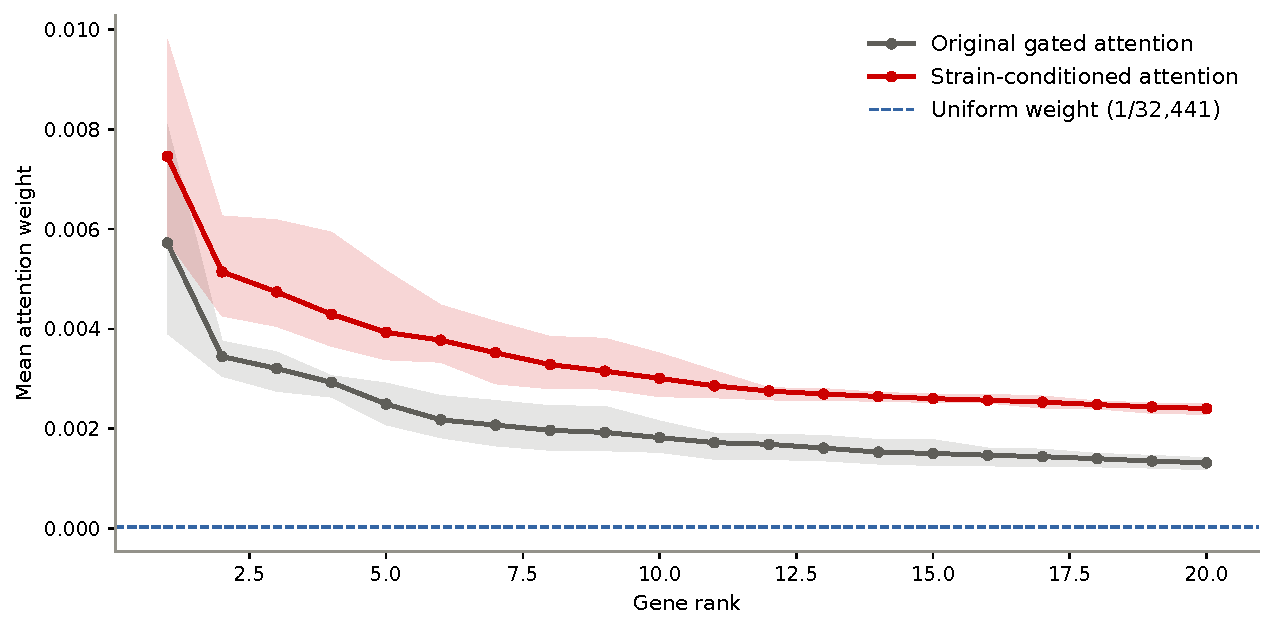
\includegraphics[width=\textwidth]{fig_attention_concentration.pdf}
\caption{Mean attention weight against gene rank in the Gene Feature Attention
Module, before and after strain conditioning.}
\label{fig:attention_concentration}
\fignote{Averaged over the seven antibiotics; the band is the range across them and
the dashed line is uniform weight over all 32{,}441 genes. The strain-conditioned
lens weights its top-ranked genes more heavily, the change
Table~\ref{tab:attnfix} records as $U_{res}$ rising from 0.0192 to 0.0419.}
\end{figure}

The strain-conditioned lens
concentrates more weight on its highest-ranked genes at every rank, and the
resistance information of the
attended genes more than doubles from 0.0192 to 0.0419, which is 89\% of the SHAP-selected genes
on average, and greater than them on five out of seven antibiotics. The focus on a
single assembly drops from 16.4-fold to 9.0-fold and three out of the seven drugs are no longer
significant in the 5\% threshold and the number of independent source assemblies between the
attended genes almost doubles, and as a result the provenance signature is mostly diluted.

\vspace{1em}

The rows of performance are not as plain as they appear at the first sight as the term buys
practically nothing where it can be measured with ease and much where it is needed. Strain conditioning is
worth almost nothing where it is easiest to measure: $+0.0024$ on the random split, and
$+0.0037$ on the full stack under the lineage holdout. It is worth an order of magnitude more,
$+0.035$, on the neural lenses alone under that same holdout, while the classical learners do
not move at all and stay at 0.628. An ablation run only on the random split would have hidden
this completely. The degenerate scoring function was costing the neural arm most of what it
lost anywhere, on precisely the split this research is interested in, and the classical arm was
strong enough that none of that loss ever showed in the headline number. Section~\ref{subsec:prevmatch}, which argues that
the classical learners carry most of this model's performance, therefore survives a version in
which the neural side is meaningfully better, a stronger form of the same argument.

\vspace{1em}

The term also changes the division of the work in the model. The gate contributes $+0.0224$
against the stacking step's $+0.0914$, a ratio of four to one; and $+0.0353$ against $+0.0679$, a
ratio of two to one. There was no change in ordering and all the antibiotics continued to improve
monotonically throughout the three stages, but about half the perceived difference between the
neural and classical halves was the result of a scoring function that was not strain-dependent.
Clinical appearance changes hardly at all: the average very major error value is reduced from
0.257 to 0.249 and the major error value is the same at three decimal places, and no antibiotic can fall
within both CLSI limits. Whatever this term is worth, it is not the reason the model is
clinically unusable.

\vspace{1em}

Our most interesting change is the one which we have not tuned for. The attention restores
MFCAOJAD\_04226, a beta-lactamase, with the score conditioned to the presence of the
strain, and selectively recovers it with ampicillin and amoxicillin-clavulanate, the two
penicillins in our panel and the two drugs which a beta-lactamase can explain being resistant to.
It is the locus tag that SHAP had already determined in the classical learners and thus, two
attribution paths that previously disagreed on all points now converge on a single gene,
independently. We do not exaggerate this: it is a single gene per hundred genes tested each lens
per drug, it is ranked 19 and 20 instead of first, and \textit{gyrA} and \textit{parC} have not
appeared in the attention rankings. It does not mean that this lens can be interpreted, since the
findings in the previous section demonstrate that, it cannot. The argument is that the standard
formulation could not have been, however much else was amiss, and that the difference can be
traced to one term in the scoring function.

\vspace{1em}

One boundary applies. This is information on the presence and absence vector for attention, and
is specific to that input, not to attention pooling in general. What generalises is that the
diagnostic is an attention mechanism whose scores do not change across samples, which means that
we cannot obtain a per-sample explanation and we can figure out that fact in minutes, without
retraining anything, from the entropy and information checks in this section. We computed the
fraction of presence-absence entropy, $U_{ST}(g) = I(g;\mathrm{ST})/H(g)$, which is equal to 1 if
a gene's presence is completely attributed to its lineage and 0 if it says nothing about the
gene's lineage. In Table~\ref{tab:umark} the selected genes are compared with the genes attended
and to 500 random selections of equal size, and Figure~\ref{fig:lineage_marker} draws the two
measures side by side.

\begin{table}[htb]
\centering
\caption{How much of each gene set is explained by lineage ($U_{ST}$) and by
resistance ($U_{res}$), over the top twenty genes per antibiotic. The attention row
is the standard formulation; the delivered strain-conditioned lens reaches 0.357
and 0.0419.}
\label{tab:umark}
\small
\begin{tabular}{|>{\raggedright\arraybackslash}p{5.6cm}|r|r|r|r|}
\hline
\textbf{Gene set} & \textbf{$U_{ST}$} & \textbf{vs.\ random} & \textbf{$U_{res}$} & \textbf{vs.\ attention} \\ \hline
Random genes (500 draws) & 0.539 & N/A & N/A & N/A \\ \hline
SHAP, classical learners & 0.375 & $0.70\times$ & \textbf{0.0473} & $2.5\times$ \\ \hline
Attention, Gene Feature Attention Module & \textbf{0.312} & $0.58\times$ & \textbf{0.0192} & N/A \\ \hline
\end{tabular}
\vspace{0.4em}

\noindent\footnotesize\textit{Note:} Attention's $U_{ST}$ of 0.312 is lower than a random gene's
0.539, so the attended genes are not a lineage marker; its $U_{res}$ of 0.0192 is less than half
of SHAP's 0.0473, so they carry far less resistance information than the genes the classical
learners select.
\end{table}

\begin{figure}[htb]
\centering
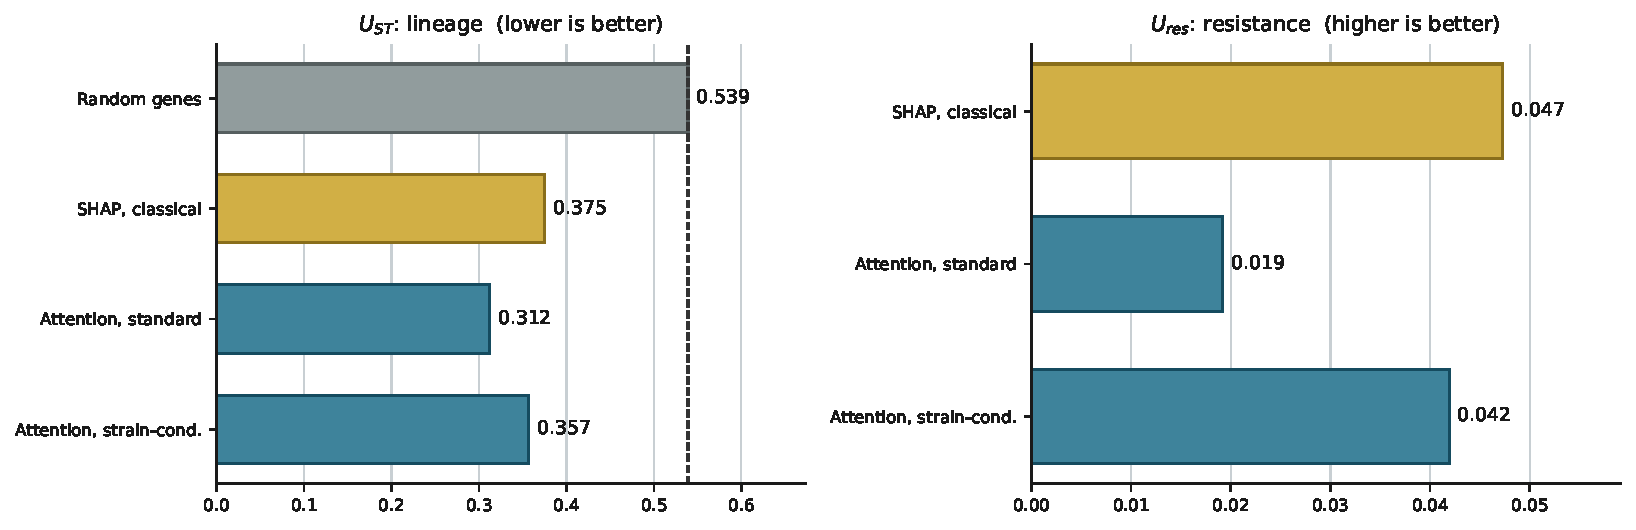
\includegraphics[width=\textwidth]{fig_lineage_marker.pdf}
\caption{The attended gene sets against SHAP on both measures.}
\label{fig:lineage_marker}
\fignote{Random draws appear on the lineage measure only, since a random gene set has
no resistance value to compare against. Lower is better on the left, higher is better
on the right.}
\end{figure}

There are two things that follow, both depicted in Figure~\ref{fig:lineage_marker}. The first is
not a feature of our model itself, but of the data: the presence-absence pattern of a random gene
from this pan-genome is explained to 54\% by sequence type. Such strongly lineage-structured
content of \textit{E. coli} accessory genes is the most obvious single reason why a
lineage-sensitive split was required in the first place.

\vspace{1em}

The second one is that the genes attended are not a lineage marker. They are \textit{less}
determined by lineage than a random gene, at 0.312 under the standard formulation and 0.357
under the delivered one, and nothing in the 500 random draws fell below them. Nor do they hold
much information of resistance: their $U_{res}$ of 0.0192 in Table~\ref{tab:umark} is the lowest
of the three sets, about half the 0.0473 that the genes SHAP chooses do, and even the
strain-conditioned version is only 0.0419. It is not the lens that read the wrong thing but the
lens that read hardly anything. Its focus is nearly even with five of the seven drugs; where it
focuses, it focuses on genes that share a provenance that does not predict either lineage or
resistance; and none of the resistance genes is in its rankings at any window we tested. The
useful part is the comparison with SHAP in that, both sets of genes were selected on the same
trained pipeline on the same features: the classical side picks genes with two and a half times
more resistance information. This matches the result reported in Section~\ref{subsec:prevmatch},
where the neural lenses alone under the lineage holdout remain at 0.472 while the classical learners
remain at 0.628. It is the same learners who generalise that are also the ones which pick the more
informative genes.

\vspace{1em}

This conflict does not exist solely on the neural side. In the classical arm, the two attribution
modes also struggle to agree to a great degree. When the top twenty genes ranked by XGBoost gain
are compared with the top twenty genes ranked by SHAP, by each antibiotic and by both sets of
classical features, the Jaccard overlap ranges between 0.053 and 0.212, with an average of 0.11 on
the gene-aggregated features and 0.17 on the raw SNP features, so at best only four to six genes
out of twenty will be shared between the two lists. The rank correlation is not so good: Spearman
is negative with all seven antibiotics, between $-0.04$ and $-0.53$. The results of two methods of
attributing to the same trained model are not expected to differ this much and hence neither can
be taken as the interpretation of the model itself. The findings of the gene level, then, are
reported as leads but not settled biology, such as the eight resistance genes above, which are
informative because they are all in agreement with independently determined biology but not
because the attribution method has ascertained them.

\FloatBarrier
\subsection{Population Structure and the Mistakes Behind the Lineage Split}

Prior to running the lineage holdout, we checked a simpler question first: the accuracy of
resistance predictions from a model able to predict from nothing but each strain's broad
phylogroup, limited to an 8-way label with no genomic context whatsoever.
Table~\ref{tab:phylogroup} reports what that baseline achieves.

\begin{table}[htb]
\centering
\caption{A baseline given only the eight-way phylogroup label, with no genomic
features, against the proposed model on the random split.}
\label{tab:phylogroup}
\small
\begin{tabular}{|l|r|r|}
\hline
\textbf{Antibiotic} & \textbf{Phylogroup only} & \textbf{TriLens-MoE-Stack} \\ \hline
AMP & 0.5562 & 0.9440 \\ \hline
SXT & \textbf{0.4144} & 0.8352 \\ \hline
AMC & 0.3606 & 0.7482 \\ \hline
CIP & 0.2452 & 0.9773 \\ \hline
CTX & 0.2015 & 0.9019 \\ \hline
CAZ & 0.1551 & 0.8299 \\ \hline
GEN & 0.1066 & 0.7037 \\ \hline
\textbf{Average} & \textbf{0.2914} & \textbf{0.8486} \\ \hline
\end{tabular}
\vspace{0.4em}

\noindent\footnotesize\textit{Note:} Trimethoprim-sulfamethoxazole's phylogroup-only score of
0.4144 sits well above its own prevalence of 0.310, the one antibiotic where broad lineage
carries real signal; the last row averages across all seven.
\end{table}

In six out of seven of the antibiotics, the phylogroup-only baseline is at or very close to the
no-skill level, which in PR-AUC is the prevalence reported in Table~\ref{tab:labels}: the excess
ranges between $-0.011$ (gentamicin) and $+0.055$ (ampicillin). Trimethoprim-sulfamethoxazole is
the exception, reaching 0.4144 against a prevalence of 0.310, which shows that broad lineage does
carry some signal for that one drug. For the other six it tells us little or nothing. This rules
out the simplest explanation of the model, namely that it works only by noticing which of the
eight broad ancestry groups a strain belongs to. The lineage holdout asks a finer-grained version
of the same question, and the answer there is different. Broad phylogroup carries virtually no signal, but fine-scale relatedness
clearly does: the specific clonal origin of a strain, in terms of hundreds of sequence types rather
than eight groups, can account for much of the model's apparent performance on a particular
antibiotic.

\vspace{1em}

One correction was needed to get the 0.634; it is a result that can easily be reproduced. We
found that the meta-learner was using the five classical learners' predictions from a file
created at construction time when the split was random, while the neural lenses' predictions were
based on the split under test. The same sizes of the splits were assigned to the random and
phylogroup-stratified splits, and nothing caused an error, simply the label of each test genome was
matched with the classical prediction of an unrelated genome. The numbers changed enough to alter
our interpretation of the result once each prediction had been matched to its genome; and now
prediction-to-genome alignment is also fixed as an initial step prior to evaluation along with the
strain-order and gene-name checks of Section~\ref{sec:data}. The moral of the story is that when
one does a split that is supposed to be more difficult, a silent alignment fault and a real lack of
lineage dependence are indistinguishable from the outside. A finding of that kind should trigger
a check of the pipeline rather than be treated as incidental.

\FloatBarrier
\subsection{The Two-Group Result: Mechanism Against Population Structure}

With the corrected split in hand, the pattern across antibiotics becomes much
clearer than it was before. The most obvious example of a learnt real mechanism is ciprofloxacin.
It also decays with a 0.030 loss when prevalence is held fixed and its two known
resistance genes are in our annotated markers. \textit{E. coli} resistance to fluoroquinolone is
typically due to point mutations in these genes: a small, precisely defined signal, and precisely
that which a model can learn once, and then recall in an unrelated isolate.
Gentamicin is the opposite case. When prevalence is fixed it still loses 0.244, the largest gap of
the seven, and no aminoglycoside-resistance gene feature enters into the final model. The
gentamicin resistance often comes on plasmid and mobile element genes and is transferred in a
lineage specific manner far more than it is across lineages, and does not assemble well in a
pan-genome built this way with this dataset. The model has learned essentially which lineage a
strain belongs to, not which gene it harbors. Lastly, ceftazidime and cefotaxime, which have losses
of 0.187 and 0.176, respectively, potentially share overlapping mobile beta-lactamase elements.

The most obvious example of another failure is amoxicillin-clavulanate that loses 0.197. The
expression of more enzyme or release of a membrane channel, changes in degree, rather than changes
in which genes are expressed, are often the basis of its resistance. This type of resistance can
never be easily overcome by our presence-and-absence lens, which bears most of the weight of the
entire gate during the course of this research, and therefore this type of resistance was never
going to be easy to capture in our design.

Two drugs in the small-gap group need a more careful word, because the mechanistic reading fits
them less neatly. Ampicillin loses only 0.017, yet its main mechanism is a TEM-1 beta-lactamase,
which is plasmid-borne and therefore mobile. A mobile gene would be expected to sit with
gentamicin rather than with ciprofloxacin. The likeliest explanation is that TEM-1 is so
widespread in \textit{E. coli} that it is no longer tied to any particular lineage. A gene
carried by half the collection behaves, for prediction purposes, like a fixed marker, whatever
its mode of transmission. Mobility alone therefore does not decide the outcome; what matters is
whether the gene is confined to a few lineages.
Trimethoprim-sulfamethoxazole is harder still, and we cannot explain it. It loses 0.031, which
places it firmly in the small-gap group, but neither our attribution analysis nor the
independent Arcadia study could identify a resistance locus for it at all
(Table~\ref{tab:arcadia}). It is also the one drug for which the phylogroup-only baseline
carried real signal, at 0.4144 against a prevalence of 0.310, which if anything ought to push it
the other way. We therefore record it as an unexplained member of the small-gap group rather
than assign it a mechanism we cannot evidence. Figure~\ref{fig:mechanism_gap} shows the
prevalence-corrected gap for all seven drugs together, which makes the size of the division
easy to see.

\begin{figure}[H]
\centering
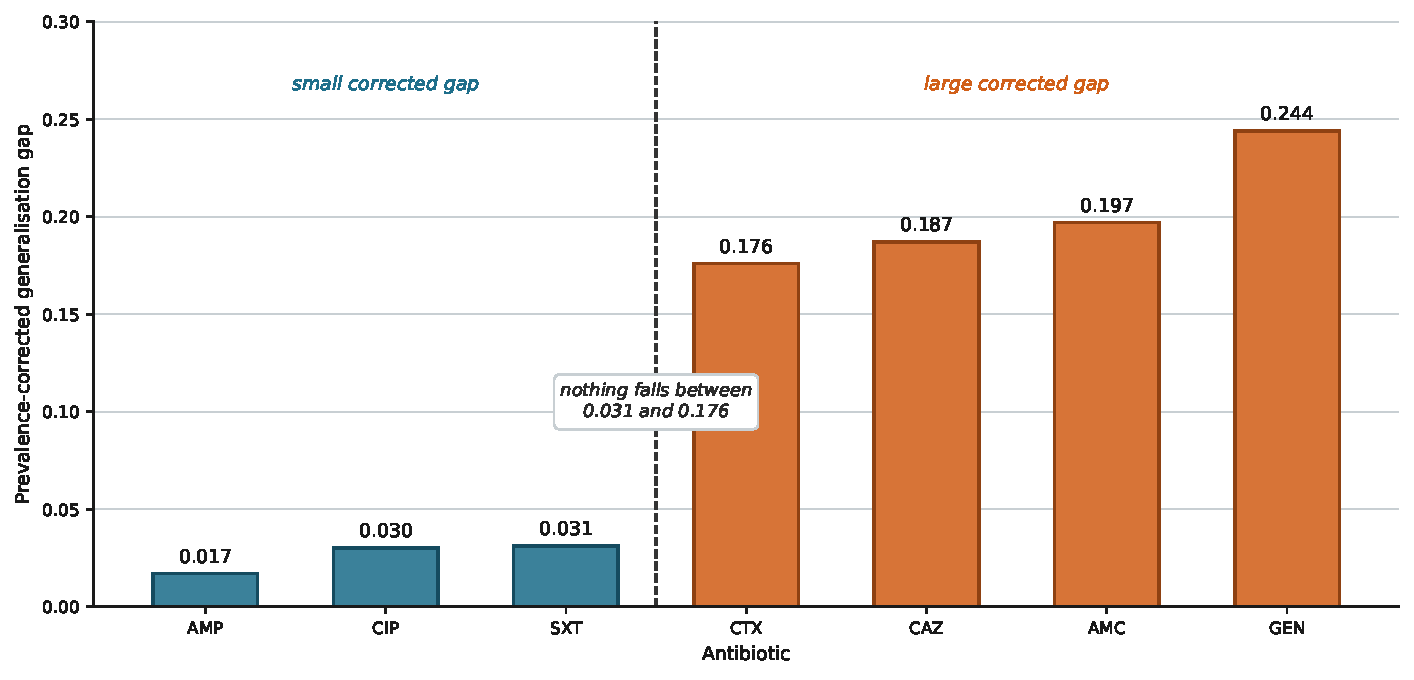
\includegraphics[width=\textwidth]{fig_mechanism_gap.pdf}
\caption{The prevalence-corrected generalisation gap for each antibiotic, ordered
by size.}
\label{fig:mechanism_gap}
\fignote{Three drugs lose almost nothing while the other four lose between 0.176 and
0.244, with no antibiotic falling between the two groups. The grouping here is
empirical; the mechanistic reading of it is set out in the text above, and it is
better supported for some drugs than for others.}
\end{figure}

All this does not make the model useless. It is efficient where the genetic basis of resistance
is stable across lineages, whether that basis is a chromosomal mutation or a gene so widespread
that lineage no longer predicts it, and inefficient where resistance rides on mobile elements
confined to particular lineages or on low level changes in gene expression. This is a specific,
falsifiable claim about the current state of genomic AMR prediction, and a more useful
conclusion than an average score would have been.

\subsection{Answering the Research Questions}

Taking the five research questions of Chapter~\ref{ch:intro} in turn.

\textbf{RQ1.} TriLens-MoE-Stack achieved an average PR-AUC of 0.849 on the random split, the
highest in Table~\ref{tab:baselines}. It is ahead of every external baseline and ahead of its
strongest component on five of the seven antibiotics, as Table~\ref{tab:vsraw} shows. But its
margin over the best single classical learner is only 0.009, which falls
within the bootstrap intervals, so the claim that can be defended is the weaker one: nothing
simpler beats it, rather than that it beats everything simpler.

\textbf{RQ2.} Each component has its contribution to make, and the classical arm has the greatest:
the addition of the gate is 0.035 and the classical step of stacking 0.068 to the random split
(Section~\ref{subsec:layerabl}). Under the lineage holdout the classical learners reach 0.628 on
their own, against 0.634 for the whole model, while the neural lenses on their own reach only
0.472, so on truly new lineages the neural side contributes almost nothing.

\textbf{RQ3.} Answered in the negative but a diagnosis was made. The gate weights can be read but
are inconsistent with the prediction of the design, diverting ciprofloxacin off of the motif lens
designed to receive it. The attention weights reclaim a single known resistance gene in 420
markers, eight in SHAP on the classical arm. Section~\ref{subsec:attnfix} shows that this failure
can be attributed to a particular and remediable attribute of the lens, an attribute more valuable
than a positive answer we cannot justify.

\textbf{RQ4.} A blend with relative proportions that change dramatically by antibiotic. Coarse
phylogroup membership has virtually no signal on its own (0.291), and gene annotation recovers
\textit{gyrA} and \textit{parC} unprompted, but the prevalence-corrected holdout indicates that
finescale relatedness has a lot: three drugs lose 0.017 to 0.031 and four lose 0.176 to 0.244, with
no results in between. There is no one answer to RQ4, just a per-antibiotic one.

\textbf{RQ5.} Partially incomplete and uneven generalisation. Average performance drops from 0.849
to 0.634 (or 0.723 after correcting for the prevalence shift) and leftover duplicates are ruled out
by a near-duplicate scan. It holds reasonably well for antibiotics with a simple well-understood
mechanism and badly for antibiotics whose resistance is linked to mobile genetic elements or to
changes in gene expression.
